
\documentclass[oneside,a4paper]{book}
%\pagestyle{headings}

\usepackage{import}
\usepackage{etoolbox}
\usepackage{graphicx}
\subimport{layers/}{init}
\usetikzlibrary{positioning}
\usetikzlibrary{3d} %for including external image
\usetikzlibrary{decorations,shapes}
\usetikzlibrary{decorations.shapes}
\usetikzlibrary{decorations.markings}
\usetikzlibrary{backgrounds}
\usetikzlibrary{calc}

\def\ConvColor{rgb:yellow,5;red,2.5;white,5}
\def\ConvReluColor{rgb:yellow,5;red,5;white,5}
\def\PoolColor{rgb:red,1;black,0.3}
\def\UpsampleColor{rgb:green,5; white,2}
\def\DetectColor{rgb:red,5; white,2}
\def\UnpoolColor{rgb:blue,2;green,1;black,0.3}
\def\FcColor{rgb:blue,5;red,2.5;white,5}
\def\FcReluColor{rgb:blue,5;red,5;white,4}
\def\SoftmaxColor{rgb:magenta,5;black,7}
\def\SumColor{rgb:green,1}
\def\LSTMColor{rgb:green,1}
\def\LSTMCLastColor{rgb:green,5}
\def\ShortcutColor{rgb:blue,3; green,1; white,5}
\def\MultColor{rgb:magenta,1}
\def\ConcColor{rgb:red,5}
\def\input_image{image/input.png}

\newcommand\highcontrast[2]{
    % Blur
    \foreach \x in {-0.05,0.05} {
        \foreach \y in {-0.05,0.05} {
            % \node[xshift=\x,yshift=\y,black!10!white] at (#1) {\large #2};
            \node[black!10!white,#2] at (\x em, \y em) {\large #1};
        }
    }
    
    % Main
    \node[#2] {\large #1};
}

% A B S T R A C T
% % % % % % % % % % % % % % % % % % % % % % % % % % % % % % % % % %
\chapter*{\centering Abstract}
\begin{quotation}
\noindent
The main goal of this project is to evaluate the application of \gls{dl} models for the classification of syllable types in recordings from the pups of the neotropical greater sac-winged bat (\emph{Saccopteryx bilineata}).
To realise this, two experiments were conducted, with the first one demonstrating how it is feasible and the second one presenting an actual realization of a prototype of an automated syllable type classification pipeline.

We aimed to classify the different syllable types of the adult territorial song and one variable juvenile syllable within variable vocal practice sequences. This was worked out in a supervised machine learning framework, where we investigated the effect of different preprocessing variants in combination with the features as spectrograms or \gls{hog}.
For the models, we considered different types and different constellations of artificial neural networks (recurrent, convolution and densely connected).

Our findings are promising and show that it is feasible to create an automated syllable type classification application in the given objective, although the syllables of the juveniles show a high degree of intra- and interindividudal variability because they mirror developmental and learning processes throughout ontogeny.
\end{quotation}
\clearpage

% Acknowledgements
% % % % % % % % % % % % % % % % % % % % % % % % % % % % % % % % % %
\chapter*{\centering Acknowledgements}
\begin{quotation}
\noindent
I would like to express my gratitude to Ahana Aurora Fernandez for providing the labelled dataset and the hours of discussion and more that formed the basis for conducting these experiments.
For their support and patience with me, I sincerely thank my supervisors Andreas Fischer and Daniel Wegman.
Thanks also to Petar Veličković, as many of the schemes on neural networks are modified versions of his publicly available work, his \href{https://github.com/PetarV-/TikZ}{TiKZ GitHub repository} was a little treasure for me.
And for providing a \gls{gpu} cluster, I would like to thanks the HPC team of UBELIX (http://www.id.unibe.ch/hpc), the high-performance computing cluster at the University of Bern, Switzerland.
And finally, I would like to thanks my friends Anna, Bettina and Sophie who all proofread my thesis.
\end{quotation}
\clearpage
\glsresetall

% C O N T E N T S
% % % % % % % % % % % % % % % % % % % % % % % % % % % % % % % % % % % % % % % %
\tableofcontents

\chapter{Introduction}
\label{ch:introduction}
A promising approach to deepen our knowledge about human language capacity is to investigate if and to what extent key components - such as vocal imitation - have evolved in other species \cite{Vernes2020}. 
These studies yield a large amount of data and the analysis of this data is time-consuming if vocalisations cannot be detected automatically. Furthermore, with complex vocal sequences consisting of several different syllable types, automatic classification of syllable types is a desirable feature.
The neotropical greatersac-winged bat species \emph{Saccopteryx bilineata} is a promising candidate for biolinguistic studies, as this species is capable of vocal imitation \cite{Knornschild2014}. 
As the study of this specific trait in \emph{S. bilineata} progresses, an increasing amount of research is devoted to the manual analysis of large amounts of bioacoustic data. More about the difficulty of manual analysis of bioacoustic data, especially syllable classification, can be found in \secref{vocalisation} and \secref{syllable_classification}.

For human speech, the understanding, parsing and encoding process is a highly studied procedure and is now used by a wide range of applications belonging to the broad field of \gls{nlp}.
Developments in this field have made it possible to convert speech directly into written form or translate it into another language in real time and many other astonishing feats \cite{Kang2020NaturalReview}. A big step for this language application came in the form of \gls{dl}, a subdivision of \gls{ml}, which emerged as a promising field.
\Gls{dl} involves the processes of "learning" information and then applying that learnt information to perform similar tasks by training deep and complex models.

% Deep learning is a subdivision of Machine Learning featuring accessible techniques for complex tasks.
\Gls{dl} tools have already been used in the field of bioacoustics. One of these applications is species identification, which uses the initial approaches of human speech decoding applications based on \gls{ml} by searching and classifying patterns in the acoustic recordings and trying to combine the results to meaningful information \cite{Stowell2019}.
Depending on the animal monitored, one was interested in the recognition of a song or only a single syllable, with the interest of distinguishing between animals.
In recent years, the number of biolinguistic studies in animals has continued to increase \cite{Vernes2020,Wirthlin2019ATrait}.
Especially in animals that are thought to be able to contribute to the study of human speech, such as the bat \emph{S. bilineata}, which comprises a promising taxon for biolinguistic studies \cite{Knornschild2014}.
This, combined with the ongoing development of computational power leveraging the analysis of more information \cite{Amodei2019}, makes the interest in applying \gls{nlp} to biolinguistics increasingly promising.
However, at the time of writing, this area appears to be largely unexplored, and no evidence of software for fully automated classification of bat syllable types has been found.


This project aims to deepen the understanding of syllable type classification of the \emph{S. bilineata} using supervised \gls{ml} on the basis of the initial \gls{dl} models used for species identification.
%This project aims to build a \gls{ml} pipeline for automated syllable type classification on the basis of the initial \gls{dl} models used for species identification.
The experiments are divided into two parts. In the first we focus on different feature preparation methods as well as insights about the performance of different \gls{ml} models.
The second part focuses on the building of a pipeline for an automated syllable type classifier prototype based on a dynamic length audio, with the generation of accessible results for further processing in other applications.
The intention behind the prototype is to construct a guide for building a more elevated classifier which uses the newly emerged techniques around \gls{nlp}.

This thesis is structured as follows. Chapter \ref{ch:background} highlights the work which contributed to the existence of this thesis. It includes a brief overview of language analysis methods and the current state of the use of \gls{ml} in this field. Chapter \ref{ch:dataset} introduces the data we used for learning (i.e. training, model evaluation and selection) and chapter \ref{ch:method} presents and discusses the methodology included in the experiments. The steps and configuration used for the results and their outcomes are described and discussed in chapter \ref{ch:experiments}.
Finally, the conclusions from the results are drawn in the first part of chapter \ref{ch:conclusions}, in the second we render the feature works.

\newpage{\pagestyle{empty} \cleardoublepage}


\chapter{Background}
\label{ch:background}
What belongs to biolinguistics, what do we know about the vocal capabilities of the bat \emph{S. bilineata} and how is this connected to \gls{ml}. This and many more insights are provided throughout this chapter.

\section{Biolinguistics}
More than anything else, language defines human nature. Language allows infinite expression with finite means \cite{Hauser2002Neuroscience:Evolve} enabling us to exchange ideas and transmit knowledge across generations, building the foundation of our technological advances and cultural heritage. However, the origins of language remain a puzzle, possibly the most challenging in science because language does not fossilize \cite{TecumsehFitch2010TheLanguage}. This renders tracing the evolution of language extremely challenging. The current most promising approach to solve this puzzle is to comparatively investigate the biological foundations of language across species \cite{Fitch2018TheAnalysis}.

The biolinguistic approach combines research methods from fields such as neurogenetics, animal behaviour, linguistics, developmental psychology, bioinformatics and mathematics to understand the underlying mechanisms and processes of human language. This make sense, as language itself is a complex system composed of several key factors (e.g. syntax, semantics, vocal imitation) and various cognitive abilities (e.g. social learning, theory of mind, recursive processing) \cite{Fitch2010SocialPhylogenies}.
Although no non-human animal communication system equivalent to the human language exists, bioacoustic research demonstrated that non-human animal vocal communication can be complex in terms of vocal repertoire size (i.e. the number of distinct syllables) (e.g. bats: \cite{Behr2004}; songbirds: \cite{Eens1989TemporalStarling}; cetaceans: \cite{Payne1971SongsWhales}), syntactical rules (i.e. the rules according to which the acoustic units – for example syllables - are arranged within vocal sequences; \cite{Weiss2014})  and vocal versatility (i.e. vocal plasticity allowing to modify existing signals and/or learning new signals from scratch based on social experience) \cite{Wirthlin2019ATrait}. Furthermore, non-human animals possess multiple cognitive skills which are required for language acquisition in the first place, such as associative learning, vocal imitation and joint attention \cite{Fitch2010SocialPhylogenies}. Therefore, the biolinguistic research in non-human animal vocal communication aims to understand if and to what extent key features and cognitive skills evolved compared to our own.

\section{Vocalisation}\label{sec:vocalisation}
Across many species, vocal communication is a common social behaviour.
Bioacoustic research seeks to uncover the structure, mechanism, behaviour and reason for vocal communication. This includes how signals are generated and perceived and how information about identity, fitness, presence of danger, environmental stress and possibly much more is transmitted. In the same way, the extent to which fitness and reproductive success are influenced by communication, is also of interest \cite{Kershenbaum2016, Manteuffel2004}.
This list is not exhaustive, thus as one can imagine, there is a large amount of unanswered questions in this field.
Unfortunately, only a tiny fraction of vocal communication seems to have been studied in detail so far. Here, the challenging work of segmenting acoustics into temporally discrete units and classifying them correctly according to specific characterising properties plays a major time-consuming, yet crucial role.

When it comes to vocal learning in non-human animals, the research field seems to be quite limited with focus on birds \cite{Petkov2012} and evidence in mammals centered around cetaceans \cite{Janik2014}, pinnipeds \cite{Reichmuth2014}, elephants \cite{Poole2005} and bats \cite{Knornschild2014}.
In recent years, researchers are debating about understanding vocal learning as a continuum rather than a dichotomy (absent vs present), including not only vocal imitation but also vocal plasticity, including the modification of innate calls based on social experience.
Martins et al. discuss the concept of a wider vocal learning continuum including more vocal abilities which are now being uncovered in other species.
Thus engaging a broader comparative study about vocal learning, as the current view seems to be too narrow and excludes vocal abilities \cite{Martins2020VocalContinuum}.

Still, non-human mammalian species which possess the ability of vocal imitation (i.e. learn a vocalisation from scratch based on the auditory input from a tutor) are especially promising candidates to study mechanisms and processes involved in language learning. Vocal imitation is a mandatory capacity for human babies and infants to acquire speech (i.e. oral output of language) \cite{Vihman2014}. One of the most important first steps in human infant speech acquisition is the canonical babbling phase during which infants acquire the phonological repertoire of the maternal language \cite{OLLER1980THEINFANCY,Vihman2014}. Infants imitate the basic speech sound subunits (i.e. consonant-vowel syllables) and refine their oral output and control over speech articulators by rehearsing syllables in sequences (e.g. "mamama", "bababa") \cite{Kuhl1996}.

\section{Vocal communication of the greater sac-winged bat}
\begin{figure}[H]
\centering
  \includegraphics[width=0.7\textwidth]{image/Sacco Dayroost.jpg}
  \caption{Greater sac-winged bats (\emph{Saccopteryx bilineata}) roosting in their day roost, the young one on the right is vocalising. The smaller bats with the dark fur are juveniles and the others with lighter fur are their mothers. (© Michael Stifter)}
  \label{fig:sacco}
\end{figure}

A highly promising candidate for comparative biolinguistic studies is the neotropical bat species \emph{Saccopteryx bilineata}.
This bat species is a vocal production learner (i.e. capable of vocal imitation) \cite{Knornschild2010} and possesses a large vocal repertoire including two song types produced by adult males \cite{Knornschild2006}. During ontogeny, pups produce long vocal sequences composed of precursors of syllable types of the adult repertoire mixed with pup-specific vocalisations. While babbling, pups acquire a part of the adult vocal repertoire through vocal imitation, namely the syllables of the territorial song \cite{Knornschild2006}. For several weeks, the precursors of the territorial song syllables gradually converge towards the territorial song of tutor males, irrespective of relatedness and pup sex \cite{Knornschild2010}.
Studying the vocal practice behavior of pups offers the opportunity to study the underlying mechanisms crucial for vocal imitation because babbling represents the oral output of ongoing learning processes. Hence, investigating acquisition of learned territorial song syllable types could serve to unravel shared mechanisms and key factors across mammalian vocal learners including humans.


\section{The value of syllable type classification}\label{sec:syllable_classification}
% more about features, which features are taken for manual classification -> methos
To gain insight about potential information encoded in acoustic vocalizations, besides behavioural observations accompanying social vocalizations to infer the context, acoustic measurements are used.
Acoustic measurements can be taken over the entire vocalization (e.g. over an entire multisyllabic call) and from acoustic units such as syllables. In general, syllables are defined as continuous sound surrounded by silence.
To measure syllables it is necessary, to detect, label and sometimes classify them.
Currently, measuring and analysing syllables in vocal sequences is an extremely time-consuming job worked out mostly manually with the assistance of audio analysis tools.
Additionally, the missing knowledge about how animals perceive vocalizations (e.g. what is the smallest meaningful acoustic unit) makes the acoustic analysis challenging. Usually, syllabic units are defined based on information of the oscillogram and spectrogram. Then, possible information encoded in vocalizations can be inferred from accompanying behavioural observations.

% Additionally, the missing knowledge about the inner processing of the auditory system of the target animals requires expert knowledge about the vocalisation and their inherent physical features, resulting in classifying the syllables on a mathematical physical basis, which then could be connected to social behaviours in additional monitoring studies.

One aspect of understanding vocal learning processes in \emph{S. bilineata} involves analyzing the acoustic parameter change of territorial song syllables across ontogeny.
This begins with the selection of these particular syllable types within babbling sequences from different individual pups at different time-points during ontogeny.
So far, this selection process is extremely time-consuming, mostly because the syllable types within vocal sequences need to be manually selected and classified based on spectral similarity to syllables from the adult vocal repertoire (i.e. babbling contains also precursors of adult syllables other than territorial song syllables), and syllable on-and offset need to be manually determined. Therefore, the automatic detection of syllable on-and offset and the classification of distinct syllable types would remarkably facilitate the analysis of acoustic datasets by significantly reducing the time dedicated to syllable selection in acoustic recordings prior to acoustic measurements.
This would result in increased sample sizes, allowing a higher number of focal individuals to be included in the analysis and increasing the frequency of sampling across ontogeny within an individual (e.g. analyse more bouts per day/week/month).
%This would result in increased sample sizes leading to higher number of focal individuals could be included in the analysis and sampling frequency across ontogeny within one individual could be increased (e.g. analyze more bouts per day/week/month).
This would enable future analysis of large datasets (big data) with temporal high resolution.

As automated classification seems to be favorable, the acoustic analysis of babbling is challenging: the gradual convergence of precursor vocalisations towards mature adult vocalisations and the high number of distinct syllable types within a vocal sequence renders automatic classification extremely difficult. Especially the gradual convergence of syllable precursors is challenging because the precursors are not exact copies of adult syllable types but vary in amplitude, duration and spectral parameters, both within and across individuals. Hence, conventional acoustic classification programs such as the template scan in Avisoft SasLab Pro quickly reach their limits.

\section{Machine learning}
During the last decade, the field of \gls{ml} has evolved at a rapid pace, reducing complexity and simplifying accessibility to the technology.
Yielding more and more interesting projects in the field biology research, which contribute again to better accessibility and growing interest for this technique in the field.
This leads to many applications in species identification. But a quite untouched area is the syllable type classification of animal acoustics for analyzing their syllable type repertoire and combinations.

According to the author's knowledge, there seems to exist no work addressing \gls{ml} on automatic classification of syllable types for any bat species. However, there exists one study where the syllable structure of the greater horseshoe bats were analyzed and \gls{ml} was employed for automated call sequence classification \cite{Zhang2019}. The syllable mining was conducted manually with the help of audio analysis software, without any \gls{ml} applied at this step.

Most vocalisation studies in animals are generally used for species classification, monitoring the health condition of the environment or the animal itself.
In a much smaller scale \gls{ml} methods are used for analyzing vocalisation, the most of these, so far, have been applied to birds \cite{Qian2017,Tchernichovski2004}, and mammals (dogs: \cite{Molnar2008}; rodents: \cite{Coffey2019}; and primates: \cite{Pozzi2010,Turesson2016}).
This reflects the current state of research, where the characterization and abstraction of vocalisation remains both an art and a science requiring typically expert knowledge. A new promising technique seems to exists in unsupervised latent models, trained on compressed structures across diverse animal vocal repertoire, and leveraged by their quantitative high throughput and ability to reveal statistical patterns in complex data of \gls{ml} methods \cite{Sainburg2020}.

Although echolocation classification could be seen as syllable type classification, we perceive this as a different task, because the interest is in distinguishing the echolocation between different species (i.e. species identification) and not between different echolocation syllables from one individual.
But as some problems overlap, the advances in this field could be a possible source of ideas.
\Gls{dl} models have been tested for detection of echolocation in audio samples (they outperformed random forest algorithms) \cite{MacAodha2018} and for classifying tropical bats based on their echolocation call \cite{Chen2020}.
Both propose a specialized version of a \gls{cnn}, where the later also uses residual paths like the ResNet \cite{He2016}.
For our project we stick to the already implemented \gls{ann} models provided by the work around classification of the Eurasian woodcock based on calls or call peaks with \gls{dl} from Gilles Waeber \cite{Waeber2019BirdLearning}. One of the applied \gls{dl} models in our work is similar to CNN\textsubscript{FULL} from the bat detective work \cite{MacAodha2018}, with some more layers. Unfortunately, the second related work was not known to the author at the time the experiments were set up and carried out, so the findings could not be included in this work.

A promising \gls{cnn} is the DenseNet \cite{Huang2017a}, originating from the field of image classification.
Huang et al. proposed densely connected convolution neural layers with reducing network parameters by reusing features.
As this type of \gls{dl} model is included in the TensorFlow framework, we included an adapted DensNet-121 in our experiments.

\newpage{\pagestyle{empty} \cleardoublepage}

\chapter{Dataset}
\label{ch:dataset}
We provide an overview of the data used and give a short statistical analysis.\\\\

The dataset used in the experiments belongs to the Free University of Berlin and is kindly provided by A. A. Fernandez from the Natural History Museum of Berlin in cooperation with M. Knörnschild, affiliated with Natural History Museum of Berlin and Free University of Berlin. It consists of acoustic recordings of bat pup vocalizations from \emph{S. bilineata} in wav-file format. The acoustic recordings were obtained over two consecutive field seasons from two populations in Panama and Costa Rica.
At each location, they were able to record the target pup in a distance of 2 to 4 meters with a high quality ultrasonic sound (\SI{500}{\kHz} sampling rate, 16-bit depth resolution). The set-up consisted of a microphone (Avisoft UltraSoundGate 116Hm, with condenser microphone CM16, frequency range 1-\SI{200}{\kHz} + 3dB) connected to a laptop (Lenovo S21e) running the software Avisoft RECORDER (v4.2.05 R. Specht, Avisoft Bioacoustics, Glienicke, Germany).
The facts that the recordings could be conducted during daytime (i.e. most of the relevant social interactions of this species occur across the day in the dayroost) with excellent visibility during the day and that the bats clearly open their mouths when vocalising, allowed individual on-axis recordings.
This, in combination with the directional characteristic of the microphone used and considering good recording conditions such as the avoidance of reverberation caused by foliage, enabled to obtain high quality recordings.

The postprocessing and labeling of the syllables were conducted with the software Avisoft SASLab Pro (v.5.2.09; R. Specht, Avisoft Bioacoustics, Glienicke, Germany).
Start and end of syllables were determined manually by researchers who have over 15 years of expertise in assigning different syllable types in the vocalizations of the focal bat species.
Assigning syllable types manually is a common procedure; for instance, babbled utterances from children are coded by human listeners without a clustering method.
As the pup syllable types show a high spectro-temporal similarity with adult syllable types from first appearance onwards, the entire adult vocal repertoire was used for visual classification of syllable types in babbling bouts.
A subset of the visually classified syllables was statistically verified by performing discriminant function analyses (personal communication AA. Fernandez).

\section{Simple call dataset}
As the syllables are manually labeled we decided for economical reasons to restrict our analyses to the syllable types of a territorial song only.
This song is composed of several syllable types of which the majority are acquired through vocal imitation by the pups \cite{Knornschild2010}. To be specific, they are B2, B3, B4 and VS as well as VSV. In addition, we included the relatively variable syllable type UPS.


\begin{figure}[ht!]
  \centering
  \begin{tikzpicture}
  \node (b2) {\includesvg[inkscapelatex=false, height=10em]{image/generated/syllable_b2.svg}};
  \node[below=-.25 of b2] {\footnotesize B2};
  \node[right=.5em of b2] (b3) {\includesvg[inkscapelatex=false, height=10em]{image/generated/syllable_b3.svg}};
  \node[below=-.25 of b3] {\footnotesize B3};
  \node[right=.5em of b3] (b4)  {\includesvg[inkscapelatex=false, height=10em]{image/generated/syllable_b4.svg}};
  \node[below=-.25 of b4] {\footnotesize B4};
  \node[right=.5em of b4] (vs)  {\includesvg[inkscapelatex=false, height=10em]{image/generated/syllable_vs.svg}};
  \node[below=-.25 of vs] {\footnotesize VS};
  \node[right=.5em of vs] (vsv)  {\includesvg[inkscapelatex=false, height=10em]{image/generated/syllable_vsv.svg}};
  \node[below=-.25 of vsv] {\footnotesize VSV};
  \node[right=.5em of vsv] (ups)  {\includesvg[inkscapelatex=false, height=10em]{image/generated/syllable_ups.svg}};
  \node[below=-.25 of ups] {\footnotesize UPS};
  \end{tikzpicture}
  \caption{Spectrograms of all six syllables which were the target of our automated classification.}
  \label{fig:syllables}
\end{figure}

\section{Descriptive statistics}\label{sec:dataset_descriptive_stats}
Our restricted dataset consists of 1276 syllables. The k-fold \gls{cv} bins contain 11 syllables, because the smallest syllable type "B4" counts only 91 samples (see \figref{dataset_sct_variable_length}).
For a brief analysis of the syllable duration, see \tabref{syllable_duration_stats}, the syllable length exhibits a high variability, with a ratio between the shortest and longest syllable of about 1:39.
To account for the differences in the counts between the syllables classes one could consider to use data augmentation methods in the data pipeline. We decided to not apply any data augmentation, mainly as it is too complex to work on sound without extensive knowledge about it physical and biological aspects in respect to the bats.

\begin{figure}[ht!]
\centering
  \includesvg[width=0.7\textwidth]{image/generated/dataset_sct_variable_length.svg}\hfill
  \caption{The distribution of the syllables from the simple call data set. Over all syllables we used 11 samples for validation and 22 for testing. The dataset is not balanced in the number of training samples, with a ratio of about 1 : 7 between the least and most represented syllable.}
  \label{fig:dataset_sct_variable_length}
\end{figure}
\begin{table}[ht!]
\centering
\begin{tabular}{l
S[table-format=3.2]@{\,\( \pm \)\,}
S[table-format=2.2, table-number-alignment = left]
S[table-format=3.2]
S[table-format=3.2]
S[table-format=3.2]
S[table-format=3]
}
\toprule
syllable type &  \multicolumn{2}{l}{mean/\si{\milli\second}} & {median/\si{\milli\second}} &   {min/\si{\milli\second}} &    {max/\si{\milli\second}} & count \\
\midrule
           VS & 13.48 &  3.78 &  13.05 &  5.20 &  24.70 &   132 \\
          VSV & 18.62 &  5.85 &  16.93 & 10.47 &  39.33 &   153 \\
           B4 & 41.19 & 15.15 &  39.06 & 16.85 &  73.19 &    91 \\
          UPS & 45.12 & 11.44 &  44.03 & 18.50 &  85.59 &   467 \\
           B2 & 59.17 & 32.16 &  49.89 & 12.98 & 200.40 &   310 \\
           B3 & 54.67 & 17.76 &  53.53 & 26.19 & 120.70 &   124 \\
\bottomrule
\end{tabular}

\caption{Descriptive statistics of the syllable durations in the simple call dataset.}
\label{tab:syllable_duration_stats}
\end{table}

\section{Terminology of syllable}
We follow the definition of previous bat and bird literature for defining a "syllable" as one continuous vocal emission surround by periods of silence \cite{Kanwal1994}, \cite{Behr2004}. They are the smallest independent acoustic units emitted from bats \cite{Behr2004}, \cite{Lattenkamp2019TheContext}.

\section{Territorial Song}
The territorial song (TS) is a multisyllabic vocalisation produced by all adult males to vocally defend their territories against potential intruders (\cite{Behr2009}). The territorial song encodes information about the males' quality, individual identity and social group membership (\cite{Behr2006}; \cite{Eckenweber2013}).

It is hypothesized, that females include the evaluation of the territorial song into their mating decision. As the males produce this song mainly at dawn and dusk\cite{Eckenweber2013}, the females should hear them sufficiently. So far, however, this has not been proven.

The TS is learned by the pups during their ontogeny through vocal imitation. This is achieved by the pups imitating the male tutors of their natal group \cite{Knornschild2010}. This is one of the main reasons for the continuing research interest in this song.

\newpage{\pagestyle{empty} \cleardoublepage}

\chapter{Method}
\label{ch:method}
From the beginning it was clear that we want to apply convolution neural networks to spectrogram input. How this could be achieved and which techniques were applied is covered in this chapter.

\section{Machine learning}
\Gls{ml} is a fast evolving software art based on statistics as well as data and computer science. It is a subdivision of \gls{ai} where computer systems run statistical algorithmic models to effectively perform specific tasks without using explicit instructions by a human expert. Instead, they are recognize and learn patterns from the data they see.
More recently, \gls{ml} models were able to master tasks that were thought to be too complex for machines, combined with the ability to perform a given task consistently and tirelessly, they could speed up the experimental process enormously and enable much broader searches for patterns. Even more exciting is the finding that in some cases, computers seem to be able to learn patters that are beyond human perception.
\Gls{ml} is now used in many fields and plays a central role in tasks such as speech recognition and translation between languages, autonomous navigation of vehicles and article recommendations.

Adapting \gls{ml} to our problem results in applying a \gls{ml} algorithm to a set of data (our recordings) and some knowledge about this data (the syllable type with their time boundaries). Through learning from the training data, the algorithm can apply what it has learned to make a prediction about the type of the syllable exhibited in a given spectrogram. The algorithm is considered to have learnt the task, when more test samples are diagnosed as the correct syllable type as a result of optimizing its parameters.
As soon as the parameter change in a learning cycle does not result in a significant impact in performance, the \gls{ml} algorithm can be seen as stable.

\section{Pipeline}
In the context of ML, the pipeline is a set of components describing the fate of the data.
It starts at the creation of the data and ends in analysing the performance of the \gls{ml} algorithm.

\begin{figure}[H]
\centering
  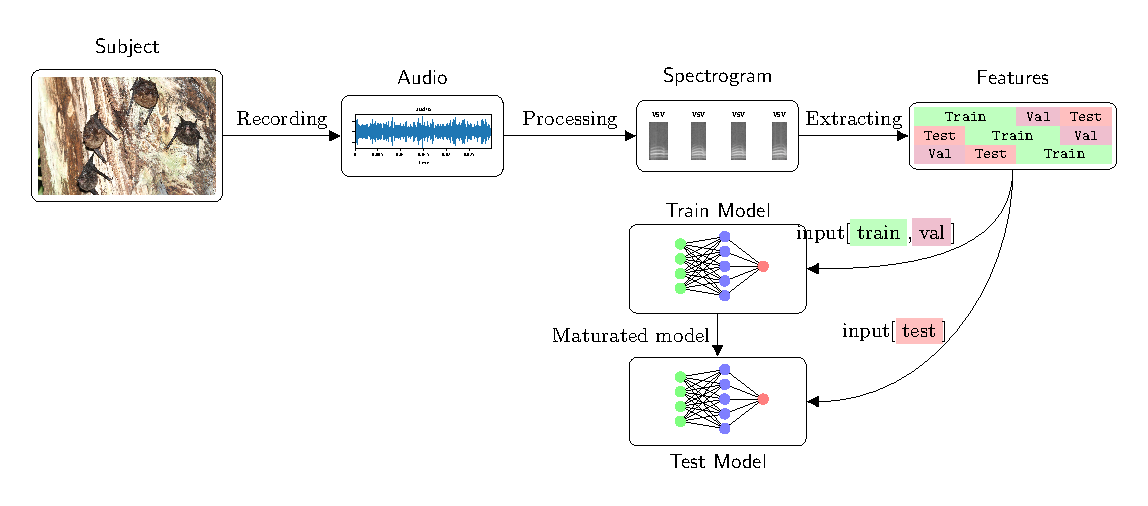
\includegraphics[width=0.9\textwidth]{plot/pipeline.pdf}
  \caption{Flow diagram of the data pipeline adapted for this project. It shows the different formats into which the data is transformed, finally it is transformed in such a way that the \gls{ml} model can understand and process it.}
  \label{fig:pipeline}
\end{figure}

\section{Data preprocessing}
Data preprocessing defines all the processing and transformations which are applied to the data before it reaches its final form that can be digested by the \gls{ml} algorithm.
Certain concepts used for data preprocessing in this project are explained below.

\subsection{Silent detection}\label{sec:silent_detection}
For noise reduction and padding of the extracted audio parts containing the syllable, we had to extract background noise from the audios.

Adapted from the librosa.effect.split \cite{McFee2020Librosa.effects.splitDocumentation}, we detect silent parts based on the \gls{rms} energy of the audio. We set the threshold to the average of the \gls{rms} energy of the audio without the syllable parts in it, as these are known foreground parts.
This leads to a conservative definition of the background audio, as this method was originally intended only for padding and thus a low-noise background audio was the goal.
The entire algorithm unfolds as follows:

\begin{equation}\label{eq:silent_detection_1}
silent = \begin{cases} 1 & mse < mean(mse \text{ without label})+1, \\ 0 & \text{otherwise}. \end{cases}
\end{equation}
\begin{itemize}
    \item As shown in \ref{eq:silent_detection_1}, the samples belonging to silent are marked with 1 in the first step and then successive samples are composed into silent slices.
    \item The silent slices are then shrunk on both sides by \SI{5}{\milli\second} and filtered against a minimum length of 10 samples. The idea behind this (which is not proven to be true for every case) is to remove the samples in the slice, where the energy becomes stronger and could lead in concatenated slices to small peaks at the beginning and end of a slice.
    \item Finally, all silent slices that overlap with a label are filtered out.
\end{itemize}
\begin{figure}[H]
\centering
  \includesvg[inkscapelatex=false,width=0.9\textwidth]{image/generated/silent_detection_sample1.svg}
  \caption{Plot of the result of the silence detection algorithm. The blackcurrant rectangles are the silent parts, on both sides the piece of \SI{5}{\milli\second} by which the silent parts were reduced is shown in transparent light blue. The yellow rectangle is a labelling part.}
  \label{fig:silent_detection_sample1}
\end{figure}

\subsection{Audio splitting algorithm}\label{sec:splitting_algorithm}
For the second experiment, with the goal of finding and classifying syllable types in an audio recording of the bats, we additionally train the network to distinguish between syllables and background.
In a comprehensive approach, we would train the network to learn the beginning and end of syllables, similar to the problems in human handwriting recognition.
Since we do not have enough knowledge in this area for this work, as well as too little capacity to learn this, we have opted for a simple version where we include background patterns in the dataset and nothing more.
For the training dataset, therefore, a preprocessing step is to split the audio and label the resulting chunks as background or as the corresponding syllable contained in the chunk.
% For analyzing a audio file containing multiple different syllable, we adapted a moving window algorithm.
This is achieved by applying a moving window to the audio source and assigning the resulting audio slices to either the corresponding syllable type or the background.
The audio slice is assigned to the corresponding syllable type as soon as a defined percentage or more of a slice is covered by a syllable or the boundaries of the syllable lie within the window, see \figref{moving_window}.

\begin{figure}[H]
\centering
  \includesvg[inkscapelatex=false,width=0.9\textwidth]{image/generated/moving_window.svg}
  \caption{Visualisation of the audio splitting algorithm with a spectrogram as background from a labelled audio file. The rectangle with the purple borders represents the moving window with the assigned labels on the upper x-axes. The yellow rectangle covers the boundaries of the annotated syllable. For visualisation reasons, we used parameters (\SI{30}{\milli\second} window length and \SI{34}{\milli\second} strides) that do not result in overlapping windows.}
  \label{fig:moving_window}
\end{figure}

For the training dataset, in order to reduce the number of slices marked as background, we discarded them after successive background slices reached three times the window length.
Ideally, this should also prevent unlabelled syllables from being marked as background, as this concept ignores slices which are a bit further away from the labels.
In the hope that there are no unlabelled syllables near labelled syllables.

\subsection{Spectrogram}
For audio analysis, the Fourier transform is one of the main tools to depict the audio and understand its inner parts. In our digital world the \gls{dft} powers all the daily used data transport with any type of signal wave, especially electromagnetic waves. The short-time Fourier transform is a multi stage process applicable on audio, this and many derivations of it allow us to generate images from signal waves in which we are able to see patterns, these images are called spectrograms.
The short-time Fourier transform determines the sinusodial frequency and phase content of local sections of a signal as it changes over time. The sampled data of a signal is divided into shorter segments of equal length and then each segment is subsequently Fourier transformed and the magnitude of the frequency spectrum of each segment is derived. The spectrum vectors are subsequently stuck together over the time axis to form the spectrogram image.

In our experiments we use a Fast Fourier transform which computes the \gls{dft} with a sufficiently good time complexity. The \gls{dft} for a fixed $N$ is the linear operator $\mathcal{F}\colon x^N \to X^N$ on $\mathbb{C}^N$ defined by:
$$
X_k = \frac{1}{\sqrt{N}}\sum_{n=0}^{N-1} x_n \cdot e^{-\frac {i 2\pi}{N}kn},  \quad k=0,...,{N-1}\in\mathbb{Z}\\
$$
For computational efficiency and not relying on the unitary transform, many implementations use the simpler scaling $\frac{1}{N}$. A unitary transform assumes that the energy in the physical domain is the same as the energy in the Fourier domain, i.e., satisfies Parseval's theorem.
% https://en.wikipedia.org/wiki/DFT_matrix#Unitary_transform

%% look up for the sox implementation

Due to the temporal segmentation of the signal, spectral leakage occurs in the Fourier transform, i.e. signal waves which are not zero at the beginning and end of the window are slightly distorted.
Since the curve of the signal at the beginning goes from 0 to the starting amplitude value (the opposite is true for the final segment), which leads to additional frequencies that are captured by the Fourier transform.
% we apply pointwise a tapering (window) function to the segmented signal...
Therefore, to smooth this behaviour, we apply a tapering (window) function to the segmented signal. We use the Hamming window in this project, it tends to fade the signal in and out at the beginning and end of the segment, resulting in an artificial periodisation of the signal within the time window length. This increases the dynamic range, but unfortunately leads to a trade-off in lower sensitivity. The Hamming window, like the Hann window, is one of the frequently used all-round windows.
The loss in information at the edges (e.g. information about transients) of the window can be reduced by overlapping the windows by some percentage. The basic idea here is that one can average FFT results form overlapping frames and thus obtain a better frequency representation of our time-domain signal.
The actual frequency resolution is still the same as without overlapping.

The resulting spectogram image thus shows us the amplitude of frequency bins over time bins. With the parameters width and height we can control the time and frequency resolution, i.e. across how many frequencies and seconds the amplitude in a pixel is averaged.
But, a signal in time and frequency domain cannot have finite support unless it is identically zero, known as the Garbor limit, based on the Heisenberg uncertainty principle, the rise in temporal resolution would give loss in frequency resolution and visa versa.
A possible solution would be a multiresolution analysis, which can give a good temporal and time frequency resolution for high, and low frequency events.

\section{Features}
When we train a \gls{ml} model, we need something to describe the subjects which the model has to learn. In the context of \gls{ml} the features can be seen as the values of the subject descriptors. They can be in many different forms, depending on the task, source, \gls{ml} and much more. In this project we use time series data in different forms extracted from an audio source.
Even the image normally contains, spatial information, and the movie extends to time, images are also able to contain the time information, as example in spectrogram images where each column represents a feature vector at time x.
As the resources are somehow limited and efficiency plays a role when a large amount of data is analyzed, one is interested in breaking down the dimensions of features to the ones which play a significant role in identifying the subjects. This can be done by the model or by an additional "hand crafted" high-level features extracting step in the data pipeline.

\subsection{Audio features}
When recording an audio, the sound is sampled at a certain rate and forms a bitstream.
The sampling rate is derived from the highest frequency to be captured by the recording, as it must strictly be more than the Nquist rate, which is twice the highest frequency.
Our recordings mostly have a sampling rate of \SI{500}{\kHz}, so we are able to capture frequencies up to \SI{250}{\kHz}.
This is more than enough to fully record the social vocalisations of \emph{S. bilineata} composed of fundamental frequencies from \SI{7}{\kHz} to a maximum of \SI{80}{\kHz}.

% which range from 5kHz to approximately 120 kHz.

As there is currently some progress in using raw waveforms as input for \gls{ml} models, we decided to transform the bitstream into some higher level features, such as the spectrogram or HOG, both of them showed good performance for different \gls{ml} models.
% references


\subsection{Raw}
In this project we call raw features a feature tensor built up from the resulting pixel values of the spectrogram image in cray scale (e.g. one channel), which are then digested by the \gls{ml} model.
This is not unique to this project, as already many researchers defined audio raw features primarily as features resulting from some Fourier transform-like transformations.
% maybe delete, thought molsty they talked about raw features like here

\subsection{Histogram of oriented gradients}\label{hog}
The \gls{hog} features are used to extract the time-frequency information from the spectrograms by retrieving the gradients present in it. This is used in a wide range of applications, such as acoustic scene classification \cite{Rakotomamonjy2015,Yang2017}, face detection in images \cite{Sun2014, Dalal2005} or videos \cite{Surasak2018}.

We use a specialisation called Slit-Style HOGs \cite{Terasawa2009}, as this was already implemented in the framework we used and provided acceptable results in combination with the \gls{lstm} model in the previous experiments from Gilles Waeber \cite{Waeber2019BirdLearning}.

\begin{figure}[H]
\centering
  \includegraphics[width=0.7\textwidth]{image/slit_style_hog.pdf}
  \caption{Visualisation of the different areas defined in the slit style \gls{hog} transformation and how they are encapsulated in each other. The slit contains $4\times2$ cells and a block is $h=2$ cells high.}
  \label{fig:slit_style_hog}
\end{figure}

Summarized, the algorithm is described as follows: The spectrogram is windowed by a slit, a rectangle of size $x\times y$, the resulting slit images are then split up in $H\times W$ cells. These cells are then assigned to blocks, in such a way that the defined blocks overlap in the height by one cell, see \figref{slit_style_hog}. Per cell the gradients are extracted in $\pi$ bins, where the gradient bins are evenly spaced over 0 - 360 ("signed gradient"). The resulting gradient vectors are concatenated together per block in a vector with a size of $h\times W\times\pi$. The block vectors are then normalized and concatenated in the slit vector resulting in a size of $((H - h + 1)\times h)\times W\times\pi$ \cite{Terasawa2009}.

\section{Deep Learning}
We give a dense overview about \gls{dl} and the \glspl{ann} used in this project, for a full explanation see \cite{Goodfellow-et-al-2016,nielsen2015neural}.\\\\

\Gls{dl} is a further subdivision of ML, this specific learning type involves the use of \glspl{ann}.
Besides the existence of different learning strategies, we focused on supervised \gls{ml}.
It involves the manual labeling of data, which is then transformed into a dataset where the connection between subject and features is given. So the problem is to approximate a function (the target function) $f\colon X \to Y$ that maps the features from some domain X to the subject in some codomain Y.
As our goal is to distinguish multiple syllable types defining our classes, the features $X$ and the subjects $Y$ are vectors with the subject information being "one-hot" encoded. The "one-hot" encoding defines encoding by assigning the class to a position in a 1d vector where the vector for a subject has the value of one at the corresponding position and the other values are set to zero, see \figref{one-hot_encoding}.

\begin{figure}[ht!]
\centering
  \includegraphics[width=0.7\textwidth]{image/one-hot_encoding.pdf}\hfill
  \caption{The "one-hot" encoding, the labels are replaced by a sparse feature vector, only the value at the corresponding position is one.}
  \label{fig:one-hot_encoding}
\end{figure}

In our case, $f$ is the function that maps an ultrasound recording slice to a syllable class, with the \gls{ann} models defined as a approximate function $\hat{f}(x, \Theta)$ parameterized by a finite-dimensional vector $\Theta^n \in \mathbb{Z}$ with some fixed $n$. The learning objective can be expressed as searching the values of the parameters $\Theta$ in a way that leads to the best possible function approximation.
The function $\hat{f}$ defines our \gls{ann} models, which is a parametric method, are bound by a fixed order or type of operations and only the values of the parameters $\Theta$ are variable.

For complex networks, learning the optimal values of the parameters is not trivial and is generally worked out by defining a cost function and stochastic optimizer algorithm.
The cost function should be adapted to the type of $y$ (and therefore to the output of the model too) and measure the extent to which the parameterized function $\hat{f}(x, \Theta)$ deviates from the target function $f$ in regard to the features from the dataset.
A suitable cost function over all datapoints is the crossentropy defined in (\ref{math:crossetropy}) describing the crossentropy between the training data $y^n$ and the model distribution, which is equivalent to the negative log likelihood.
\begin{equation}
    C=-\frac{1}{n}\sum_i^n\left(y_i\ln{\hat{y}}+(1-y_i)\ln{(1-\hat{y}_i)}\right) \label{math:crossetropy}
\end{equation}
The convention is that $0\ln{0} = 0$ but $\hat{y}\ln{0} = \infty$ for $\hat{y} \neq 0$ makes the loss function perfect for binary classification tasks.
For our multi-class classification task we took the categorical crossentropy loss function, it is the sum over $C$ classes from the crossentropy between the "one-hot" encoded training data and one model prediction of the same length, where the model prediction is normalized by a prepended softmax layer.
$$
L(y,\hat{y}\mathit{\_softmax}) = -\sum_{c=1}^Cy_c\ln{\hat{y}\mathit{\_softmax}_c}
$$
The softmax function is introduced in the next section \ref{sec:ann}.

A basic stochastic optimizer used for \gls{dl} is the \gls{sgd} algorithm. This algorithm alters the model parameters by specific proportions in respect to the gradient value of the cost.
$$
\Theta := \Theta - \eta\nabla J(\Theta)
$$
The proportion is defined by the learning rate $\eta$, this hyperparameter should be carefully tuned as it affects time and quality of the solution it converges to. A more sophisticated type of optimizer is the \gls{adam} algorithm, which is the one we use for our experiments.
Compared to the \gls{sgd}, it provides an adaptive learning rate per parameter and uses moments of the stochastic gradients to calculate the resulting values. The moments lead to smaller changes in direction.
One can imagine a ball entering from one side at the top of a valley and rolling downwards.
Due to the built-in moment calculation, the ball rolls straight down the valley after some zigzag movements, as if some force tries to keep the ball in the middle of the valley.
How much the forces of the moments influence the direction is controlled by the hyperparametres beta1 and beta2, which are the exponential decay rate of the first and second moment estimates.
Although \gls{adam} is controlled by three hyperparameters: learning rate, beta1, beta2; it is often sufficient to set the learning rate and the other two can be left at the default value.
As the learning objective has not changed, we used the same parameters as the framework provided.

These two algorithms are used in conjunction with the backpropagation algorithm.
For explanation, let us first consider the forward pass algorithm, which describes the first part of the training.
The forward pass of a simple feedforward network with three layers can be described in a mathematically simplified way with the chain rule $f(x)=f^{(3)}(f^{(2)}(f^{(1)}(x)))$, this implies that each layer is described by a function $f^{(d)}$. The first derivative of this function can be written out using the chain rule as follows $\frac{\partial f}{\partial x}=f^{(3)'}(f^{(2)}(f^{(1)}(x))f^{(2)'}(f^{(1)}(x))f^{(1)'}(x)$. It can be seen that the gradient calculation involves some repetitive calculations, e.g. $f^{(1)}(x)$. Such results are calculated and cached during the forward pass, this concept of caching intermediate results is called dynamic programming.
Then for "learning" the parameters, the backpropagation algorithm populates the error computed by the loss function back to the input layer and solves the partial derivative $\frac{\partial C}{\partial p}$ layer-wise, which results in the parameter gradient in respect to the error. Subsequently, leveraged by the stochastic optimisation algorithm, the corresponding gradient is applied to each parameter.

\subsection{Artificial neural networks}\label{sec:ann}
The \gls{ann} functions by imitating the neural connections made in the biological brain and connected these in a network of nodes, forming multiple layers.
In the \gls{mlp} architecture nodes are called perceptrons or neurons and are the computational units. The parameterized scalar valued function takes a set of inputs $x_1,\hdots,x_n$ and transforms the values by some parameters to the output $y$. The basic parameters are the weights $w_1,\hdots,w_n$, one for every input and the bias value $b$, through them one controls what the neuron computes. The processed input is given to an activation function (transfer function) $\sigma$ which is commonly a threshold function.
\begin{equation}
    y=\sigma\left(b + \sum\limits_{i=1}^{n}{x_iw_i}\right) \label{math:neuron}
\end{equation}
The math in a neuron is defined in (\ref{math:neuron}), which is an affine transformation of the input fed into an activation function.

\begin{figure}[H]
\centering
  \includegraphics[width=0.9\textwidth]{image/mlp_schema.pdf}
  \caption{A diagram of a single perceptron, along with its position within a multilayer perceptron with fully connected layers.}
  \label{fig:mlp_schema}
\end{figure}
The \figref{mlp_schema} shows the structure of an \gls{mlp}, the neurons are stacked in layers, with sparse to fully connected neurons between the layers. The number of neurons per layer can vary and activation functions can normally change per layer. Basically, called as the "feedforward \gls{ann}", the layers are connected in an order, starting with the input layer which digests the provided features. This is then followed by one or more hidden layers, hidden because their activation is hidden from the outside, and in the end there is finally the output layer (a.k.a. classification layer). The output of a neuron is digested by the neurons of the next layer sequentially, thus the activations are only passed on to the subsequent layers.
This combination of neurons supports the aggregation of information from neurons specialised in the analysis of a single element to neurons at higher layers analysing more complex information.

The type of activation function and its respective abilities plays a crucial role for mapping complex functions, for example, a composition of linear functions is again a linear function, this implies that a \gls{mlp} with only linear functions as activation functions will decay into a single layer network handling linear tasks.
By selecting them consciously, they power the rise of the \gls{mlp} networks by granting them the ability to learn non linear boundaries.

\begin{figure}[ht!]
\centering
  \includegraphics[width=0.7\textwidth]{image/activation_functions.pdf}\hfill
  \caption{Graphs of some activation functions used in ANN.}
  \label{fig:activation_functions}
\end{figure}

One of the first class of functions commonly used were sigmoidal functions such as the logistic function $\sigma(x)=\frac{e^x}{1+e^x}$ and the hyperbolic tangent function tanh. In recent years the computationally cheaper rectifier function $\sigma(x)=max(0,x)$ called rectified linear unit (ReLU) has become the most used function for deep neural networks \cite{Lecun2015}.
This function has the advantage over the sigmoid function, that the weights for large values do not become insignificant e.g. changing them influences the input in a linear manner as long it is over the threshold.
Because of this, the ReLU is seen as a possible approach to address the vanishing gradients problem when training deeper models.
For multi-class problems, the softmax function is commonly used for the output layer. The normalising exponential function is defined as $\sigma(x)_i = \frac{e^{x_i}}{\sum_{j=1}^C e^{x_j}}$ for $C$ classes, it is a generalization of the sigmoidal function for multiple dimensions. The calculated values can be seen as probabilities of how likely the network is to classify the input as one of the classes.

%
%Batch normalisation???? Goodfellow et al
%

\subsection{Long short term memory}
\Gls{lstm} architecture contains cells with a inherent state unit and the \gls{lstm} cells belong to the \gls{rnn}.\Glspl{rnn} are specialized networks to analyze sequence data. The \gls{rnn} cells hold a inner state, which influences the reception of the next value.
Because the basic \gls{rnn} cell does not control the alteration of the inner state, it tend to quickly "forget" information.
The \gls{lstm} cell, as the name implies, exhibits memory gates that control the values that update the internal state, which increases the memorization ability.

\begin{figure}[H]
\centering
  \includegraphics[width=0.7\textwidth]{image/lstm_schema.pdf}
  \caption{A diagram of a single \gls{lstm} cell and which values are recurrently used when processing a feature vector $x_1,\hdots,x_n$.}
  \label{fig:lstm_schema}
\end{figure}

The upper diagram of the \figref{lstm_schema} shows the inner parts of a typical \gls{lstm} cell. The previous output value and the new input value are both used by all gates to determine which part of the values should be changed.

The gates function by squeezing the values between 0 and 1 (usually the transformation function is a sigmoidal one), the resulting output is then multiplied point-wise by the destination vector, resulting in a down-regulation of some elements in the destination vector. The forget gate, for example, controls what is overwritten (what should be forgotten) in the state value. The input gate is a special case because it is the same function as the one used by the activation function.

The lower diagram exibits how the cell processes an input vector $x_1,\hdots,x_n$, where the current state $c_t$ and output $y_t$ is used for analyzing the next element. An elaborated and easily understandable description of the \gls{lstm} cell is provided by Christofer Ola on his blog \cite{Olah2015}.

\subsection{Convolution neural networks}
The \glspl{cnn} are a kind of deep neural networks tailored for image-like data and inspired by the behaviour of the animal visual cortex. They consist of convolution layers, containing a tensor of filters, where the values of the filters are the trainable parameters.
The filters are convolution kernels, a one or more dimensional matrix, which becomes convoluted over the input in a windowing manner.
% Similar the process can be adjusted by the padding and stride, depending on the configuration it leads to a bigger or smaller output.
The output of the convolution layer is then sent through an activation function.
\begin{figure}[H]
\centering
  \includegraphics[width=0.7\textwidth]{image/cnn_schema.pdf}
  \caption{A diagram of a single convolution layer depicts the fate of the features through them.}
  \label{fig:cnn_schema}
\end{figure}

Overall, a convolution layer is entirely defined by four hyperparameters; the number of kernels $k$, their spatial extent $v$, the strides $s$ and padding $p$. Given an input of $[W_1, H_1, D_1]$, the corresponding convolution layer output $[W_2, H_2, D_2]$ relates to the input one as follows:
$$
W_2 = \frac{W_1-v-2p}{s+1}; \quad H_2=\frac{H_1-v-2p}{s+1}; \quad D_2 = k
$$
In our experiments we stick to the already implemented variants of hyperparameters v=3, s=1 and p=1 which seems to be a common choice \cite{Huang2017a, Simonyan2015}.

Compared to a layer in the \gls{mlp}, the neurons are quite similar, they are composed of weights, a bias and an activation function. The difference is, that the convolution neuron shares the activation function and only has a constrained set of weights per layer. This "constraint" allows the convolution layer to detect a characteristic, spatially local pattern in his receptive field, of the input data over the whole input at different places. Additionally, the stacking of convolution layers leads to non-linear filters that become responsive to larger regions of input space, so the networks creates representations of small parts (the receptive field) which are assembled to representations of larger areas.

\subsection{DenseNet}\label{sec:denseNet}
\begin{figure}[ht!]
\centering
  \includegraphics[width=0.5\textwidth]{image/denseNetBlock.jpg}
  \caption{Densely connected convolutional network block with 4 weight layers and a growth rate of 4. (© \cite{Huang2017a})}
  \label{fig:denseNet_block}
\end{figure}

The DenseNet takes advantage of the concept of additional connection by passing on layers, as other deep networks like ResNet. This idea stems from a problem which arises around deep networks; when continuously adding layers the performance saturates at some point. When adding more, e.g. increasing network depth beyond some point, it results in a significant drop in accuracy.
This concept of additional skip connections allows networks to be employed with more than 100 layers in a efficient manner.
In contrast to the skip connections from the ResNet, the DenseNet applies a dense connectivity pattern where the feature map of a layer $l$ is passed to all $L-l$ subsequent layers. This is worked out block-wise by concatenating the output of all previous layers as input to the next layer. Where a layer is a combination of convolution layers and max pooling.
As a direct consequence of the input concatenation, the feature maps learned by any of the
DenseNet layers can be accessed by all subsequent layers per block. This encourages feature reuse throughout the network, and leads to more compact models \cite{Huang2017a}.
Besides this, there are some evolving concepts incorporated, like bottleneck and full pre-activation \cite{He2016a}.
In addition, because of the skip connections, one can reduce the memory of the network with some nice tweaks like sharing the memory for outputs between the subsequent inputs in a dense block \cite{Huang}.


\subsection{Regularization}
The \gls{ann} network architecture used in the experiments constitutes a complex computational model, which incorporates a high number of parameters. With the limited data we have, this makes the network prone to overfitting. Fortunately, the field of \gls{ann} has an arsenal of regularization techniques to prevent overfitting, we present the ones used in our models.

% https://link.springer.com/article/10.1007/s11042-019-08453-9
With Dropout, the \gls{ml} model randomly drops units from the network during training, which corresponds to an activation of zero \cite{Srivastava2014Dropout:Overfitting}. For every training example digested by the network the input or neurons are randomly dropped with probability $p$ resulting in a thinned input and a thinned network. This forces the model to create alternate decision paths and hopefully simpler ones. The backpropagation of the training step then only concerns the parameters of the thinned network (respectively the retained neurons and inputs), which leads to the training of an ensemble of thinned networks. After a training step, when evaluating the model on the validation set, the full model without dropout is used. To account for the scaled weights of the neurons to which dropout is applied, the weights are multiplied by the probability $r=1-p$, i.e. the probability that they are retained in the network. This should grant that for any involved neurons the expected output at training time should be equally to the output at test time \cite{Srivastava2014Dropout:Overfitting}.

Max pooling has some regularization abilities, but this is not the main focus of this concept.
The pooling layer is commonly combined with a convolution layer at the front and it subsamples its input tensors into a smaller output tensor. The subsampling is applied to every channel, therefore the resulting tensors only vary in width and height where the channel stays the same. The subsampling is done in a sliding window manner where the values of a window are sampled in respect to the pooling operation. Common pooling operations are max, average or $L^2$-norm and common hyperparameters are $2\times2$ for patch size and strides.
One advantage of applying a pooling layer to a feature layer is that the features are invariant to small spatial shifts. This can be useful when detecting the presence of a pattern is more important than determining its exact position. Unfortunately, this nice feature leads to the loss of some information in the layer.

\section{Evaluation}
\Gls{ann} can be difficult to understand, as their inner workings become, in a way, obfuscated by the large number of units. Compared to SVM or other similar \gls{ml} models it could be near to impossible to explain the effect of a unit on the network, e.g. knowing which changes of the hyperparameters leads to which exact outcome.
Therefore, we use tools for evaluating the models in a way that we can understand the inner working in a broader view. In this chapter we will introduce some methods to train and evaluate \gls{ann} models.

\subsection{K-fold cross-validation}
%https://stats.stackexchange.com/questions/27730/choice-of-k-in-k-fold-cross-validation
%https://stats.stackexchange.com/questions/61783/bias-and-variance-in-leave-one-out-vs-k-fold-cross-validation?answertab=votes#tab-top

A model validation method is used for measuring the extent to which a model generalizes, e.g. how good it performs on unseen data.
The generalisation can be assessed by comparing the predictions from the unseen data with the true output.\\\\

K-fold \gls{cv} is a model validation method and is a general tool for selecting models on datasets with difficult-to-check assumptions on the data generating process \cite{Zhang2015}.
It is preferred over other methods when the dataset has limited samples, as it run the model on the whole data, with the trade-off that multiple runs are conducted per dataset and \gls{ml} model.
As the name of the method already implies, the experiment is executed $k$ times.
The data is evenly spread over $k$ bins, with the shortest classes defining the bin size. The remaining samples are added to the training set.
In every round the model is trained on $k-v-t$ bins plus the remaining samples, where $v$ is the number of validation bins and $t$ is the number of testing bins used. After each run, the bins are shifted by one, so that all subsets contain every bin at least once.
\begin{figure}[H]
\centering
  \includegraphics[width=0.7\textwidth]{image/k-fold_cv.pdf}
  \caption{A visualisation of the distribution of bins in a k-fold \gls{cv} with $k=4$, using one bin each for validation and testing.}
  \label{fig:k-fold_cv}
\end{figure}
In the context of this method we speak about two different estimations made on unseen data. One is during model maturation where the unseen data belonging to the validation set is used for picking the model in the best state. The other (belonging to testing) provides a fair assessment on the maturated model, after the test, no changes on the (hyper)parameters should be made anymore.

% https://link.springer.com/chapter/10.1007%2F978-3-319-44636-3_4
An additional input about model generalisation is provide by Juan Gabriel Colonna et al. \cite{Colonna2016}.
They propose to include the species and specimen information at the split process in a way, that syllables of one specimen are in test or validation only. This enables the assessment of how well the model is generalized for detecting syllables of new specimen of the same species. As we are interested in the performance on different feature presentations, we omitted this kind of preparation. In a future work, the integration of species and specimen information would become interesting!

% mit andreas besprechen

In our experiments, the samples were stratified by their labels and then distributed evenly to the bins depending on their input order, in contrast to the basic concept where the samples are distributed in a randomized manner. We chose this concept because it ensures that samples of the same audio are more likely in the same bin than distributed over all bins, which should result in a more accurate estimation on how the model could generalize as the validation and test bins are less likely to contain a sample of the same audio as a sample exiting in the training bins.
However, due to this decision, we loose the nice feature of randomization, which helps to break preexisting order of datapoints and ensures a similar distribution as possible.

\subsection{Learning curves}
% https://www.baeldung.com/cs/learning-curve-ml
We already showed how the training is done in this project, but how do we assess this? And how is this used to select the interesting model, i.e. parameter set?\\\\

During the training phase of a model one can monitor the loss and accuracy of the \gls{ml} model on the training set and the validation set. The resulting visualisation graphs of loss or accuracy over time belong to the learning curves, they are widely used as diagnostic tools for \glspl{ann}, as they learn from the data set in an incremental manner.

The training curves provide information about how well and quickly the model can learn from the data.
If the model is too simple (e.g. small \gls{ann}) the model tends to struggle with the learning data, called underfitting. As the model is unable to capture the patterns in the training data, the accuracy plateaus at low magnitude and the loss remains relatively high.

\begin{figure}[ht!]
\centering
  \includesvg[inkscapelatex=false,width=0.9\textwidth]{image/generated/train_val_cnn_1d_sct_compressed_nrs0_raw_100.svg}\hfill
  \caption{Visualisation of the training curves exibiting overfitting, with the accuracy and loss curves merged into one plot. The validation loss draws a U-shaped curve with a increasing gap to the training loss and the training accuracy is about 10\% higher than the validation accuracy.}
  \label{fig:train_val_cnn_1d_sct_compressed_nrs0_raw_100}
\end{figure}

By considering all four graphs, one can extract information about overfitting and how the validation data is represented by the testing data and vice versa.
Overfitting becomes visible by plotting both accuracy graphs together. Where over time the gap between the greater training accuracy and lower validation accuracy becomes visible.
Commonly, this gap increases over time, as the model starts to over optimize more and more to fit to the training data.
The overfitting behaviour is also visible when comparing the two loss curves, with the training loss curve getting steadily lower and the validation loss curve initially decreasing until it starts to increase, sometimes exponentially, resulting in the typical U-shaped curve.

Consider an accuracy and loss graph from the validation data, one option would be to select the epoch with the lowest loss value, but as we are more interested in the accuracy and the loss value is typically only used as a proxy for the accuracy, the better choice is to select the model where the validation accuracy stops improving. But when does accuracy stop improving? One can say this happens when the accuracy starts to plateau the first time or starts fluctuating around the same value for some epochs. It could happen that if we train over many more epochs after the accuracy starts to plateau, that it increases again, but the magnitude would likely be small and therefore be negligible \cite{nielsen2015neural}.
As this seems to be a valid point, there exists a different view; Goodfellow et al. suggest in the book deep learning \cite{Goodfellow-et-al-2016} to select the model with the lowest validation loss, as the generalization is then typically maximized.

Therefore, we tend to take one snapshot of the epoch with the lowest validation loss and one with the highest validation accuracy. Finally, in the results, we stick to the second metric because of our interest in comparing the accuracy.

% andreas

\subsection{Layer wise relevance propagation}\label{sec:evaluation_lrp}
% https://towardsdatascience.com/indepth-layer-wise-relevance-propagation-340f95deb1ea
% https://git.tu-berlin.de/gmontavon/lrp-tutorial
% https://lrpserver.hhi.fraunhofer.de/

For image-like features, there is a well-suited technique called \gls{lrp}.
After a forward pass, the algorithm searches neurons that contribute most to the result backwards through the network.
This is done by examining the weights and activations from the forward pass. The contribution of a neuron is significant if it has a high activation value and it contributes to a lot to relevant neurons in the deeper layers.
The result can then be visualised as a heat map where the areas with high pixel values are the most important for getting a certain result.
Unfortunately, the python framework ”innvestigate” used to explore the \gls{dl} model was not fully supported by the TensorFlow version used.
Therefore some changes were made with insufficient knowledge about the code of the framework in question, in the hope that they would have limited damage on the results. Thus, when interpreting the results they should be taken with a pinch of salt.

\newpage{\pagestyle{empty} \cleardoublepage}


\chapter{Experiments}
\label{ch:experiments}
At first we provide a brief intro about our setup, including the used software, preprocessing, \gls{dl} models, and applied parameters. Secondly we cover the experiments, which are divided into two parts:
\begin{itemize}
    \item \textbf{Test experiments}: We try to understand how in general the \gls{dl} models could classify only the syllables, without additional background samples.
    \item \textbf{Seq experiments}: We investigate the \gls{dl} models' performance on detecting syllables by providing the whole audio as slices in a moving window manner.
\end{itemize}

\section{Main setup}
This chapter contains the general experiment set-up. Specialisations are described in the additional subchapters in the individual experiment chapters if required.

\subsection{Software}
We adapted a piece of software created with the bachelor thesis "Bird Voice Deep Learning" \cite{Waeber2019BirdLearning} kindly provided by Gilles Waeber.
Apart from needing a similar pipeline and \gls{dl} models to conduct our experiments, it provides some interesting features like interruption awareness and extended logging of the results in an accessible manner.

\subsubsection{Changes}
We removed the birdvoice\_server section of the code and everything else needed to run the web application.
The Docker files we kept back, but they would first have to be adapted to the new folder structure.
Since UBELIX, the HPC cluster at the University of Bern, does not directly support docker, we did not further invest in it.
Moreover, due to the possibility of installing our custom software on UBELIX, we no longer needed this or similar options.

Then we updated to TensorFlow 2.3, as with this version we could use the Ragged Tensors for variable length input data.
This allowed us to train the \gls{lstm} model through the convenient training method from Keras-Model including batch and \gls{gpu} support. Therefore, we could ignore all the specialized parts of the software written for training the \gls{rnn} models with variable length input.

For portability reasons, all file paths are made relative to the data path and converted to slash delimited paths which are written to reports or similar reused data files.

We used the jupyter notebook library for generating reports about the experiment testing results. The reports are generated by a template which can be customized as needed.

\subsubsection{Dependencies}
Over time and with the advent of new products or simply through convenience, the dependencies have changed a little.
The changes are presented below:
\begin{itemize}
    \item Python 3.8, although unfortunately we do not make direct use of new features such as the walrus operator.
    \item TensorFlow, this version enables faster \gls{lstm} training, as it fully supports the concept of Ragged Tensor.
    \item innvestigate\@updates\_towards\_tf2.0, with some additional modifications, we could use the "innvestigate" library in conjunction with TensorFlow 2.3 for generating the \gls{lrp} headmaps by the deeptalyor algo.
    \item Wavinfo 1.6.2, is used for extracting the label information produced by the avisoft software.
\end{itemize}

\noindent
Below are the relevant python libraries:
\begin{itemize}
\pyLib{TensorFlow GPU 2.3.1}{https://www.tensorflow.org/}{machine learning backend}{Apache 2.0}{https://github.com/tensorflow/tensorflow/blob/master/LICENSE}
\pyLib{Numpy 1.19.1}{https://numpy.org/}{fast numeric computation}{BSD-3-Clause}{https://github.com/numpy/numpy/blob/master/LICENSE.txt}
\pyLib{TQDM 4.50.2}{https://github.com/tqdm/tqdm}{progress bars}{MPL 2.0}{https://github.com/tqdm/tqdm/blob/master/LICENCE}
\pyLib{SciPy 1.5.3}{https://scipy.org/}{linear algebra}{BSD-3-Clause}{https://github.com/scipy/scipy/blob/master/LICENSE.txt}
\pyLib{Matplotlib 3.3.1}{https://matplotlib.org/}{2D plotting}{PSF}{https://matplotlib.org/users/license.html}
\pyLib{FileLock 3.0.12}{https://github.com/benediktschmitt/py-filelock}{file locking}{Unlicense}{https://github.com/benediktschmitt/py-filelock/blob/master/LICENSE}
\pyLib{Jupyter Notebook 4.6.3}{https://jupyter-notebook.readthedocs.io/}{interactive notebooks}{BSD-3-Clause}{https://github.com/jupyter/notebook/blob/master/LICENSE}
\pyLib{Librosa 0.8.0}{https://librosa.org/doc}{manipulate audio}{ISC License}{https://github.com/librosa/librosa/blob/main/LICENSE.md}
\pyLib{Wavinfo 1.6.2}{https://wavinfo.readthedocs.io}{read wav labels}{MIT License}{https://github.com/iluvcapra/wavinfo/blob/master/LICENSE}
\end{itemize}

\subsection{Spectrogram}
\begin{itemize}
\item The spectrograms have been created with SoX using the audio recordings.
\item Sampling rate is set to \SI{500}{\kHz}.
\item Height is variable, no band-pass filtering (0-\SI{250}{\kHz}).
\item All other parameters vary per experiments.
\end{itemize}

\subsection{Samples}
\begin{itemize}
\item The models were trained by k-fold cross-validation with k = 8, validation bins 1 and testing bins 2.
\item The samples are distributed among the bins so that each bin contains the same number of samples for each class. The remaining samples are always used for training and therefore do not change between runs.
\end{itemize}

\subsection{Features}
\begin{itemize}
% normalizing is more mean 0 and sd +-1 or putting different variables on a common scale.
% -> scaling fits here more
\item Raw stands for pixel features from the spectrogram scaled between 0 and 1. % the scale is because of the matplotlib
\item For \gls{hog} features, the descriptors are extracted by HWRecog (without preprocessing) using the Slit-Style \gls{hog} variant.
\item The \gls{hog} variant suffixed with 3D, the 12 bins of the HOG-descriptor are populated to 12 channels/layers of the image.
\item The values are normalized for each sample between -1 and 1.
\end{itemize}

\subsection{LSTM Model}
\begin{figure}[ht!]
\centering
  \includegraphics[width=0.9\textwidth]{image/model/ml_model_lstm.pdf}\hfill
  \caption{Visualisation of the \gls{lstm} architecture. The size of the elements does not correspond exactly to their real dimension numbers.}
  \label{fig:ml_model_lstm}
\end{figure}

The \figref{ml_model_lstm} represents the \gls{lstm} architecture used for the experiments. Form left to right:
\begin{itemize}
\item Input layer, it provides raw or \gls{hog} features in various sizes.
\item First \gls{lstm} layer with 265 neurons, it transmits the whole output sequence to the next layer.
\item Second \gls{lstm} layer with 265 neurons. Only the output of the last element is transmitted.
\item Two fully connected layers with 1024 neurons and a dropout rate of 50\%. Both use the ReLU activation function.
\item The final classification layer is a fully connected layer with softmax activation.
\end{itemize}

\subsection{CNN Model}
\begin{figure}[ht!]
\centering
  \includegraphics[width=0.9\textwidth]{image/model/ml_model_cnn.pdf}\hfill
  \caption{Visualisation of the CNN architecture. The size of the elements do not correspond exactly to their real dimension numbers.}
  \label{fig:ml_model_cnn}
\end{figure}

The \figref{ml_model_cnn} represents the CNN architecture used for the experiments. Where the CNN 1D model uses 1 dimensional convolution layers. From left to right:
\begin{itemize}
\item Input layer, it provides raw or \gls{hog} features in various sizes. % dimensions or sizes???
\item The next five blocks consist of a convolution layer followed by a max pooling layer with ReLU activation function.
The size and stride of the pooling layer are $2\times2$, resulting in dividing the size of the volume and the number of feature maps in half.
From the second block onwards the next block is only created if the output shape of the previous block is big enough.
The filter configurations of the convolution layer in the blocks are as follows:
    \begin{enumerate}
    \item $32\times3\times3$
    \item $64\times3\times3$
    \item $64\times3\times3$
    \item $128\times3\times3$
    \item $256\times3\times3$
    \end{enumerate}
\item The output of the previous max pooling layer is flattened (sample dimension reduced to one) and transmitted to a fully connected layer with 1024 neurons, a dropout rate of 50\% and a ReLU activation function.
\item The final layer, also called the classification layer, is a fully connected layer with the same number of neurons as classes. The classification layer uses the softmax activation function.
\end{itemize}

\subsection{DenseNet Model}
We use the DenseNet-121 architecture as described here \cite{Huang2017a} followed by a a fully connected layer with 1024 neurons, a dropout rate of 50\% and a ReLU activation function. The final classification layer uses the softmax activation function.

\section{Test experiments}
The general aim of these experiments is to understand how the models performs on different preprocessed syllable samples. Therefore, we only altered the preprocessing hyperparameters for the different tests.
However, one should be aware that the gls{dl} models are automatically adjusted to the size of the input data, which leads to a change in the number of parameters of a gls{dl} model.
Whenever possible, we tested the resulting features on all \gls{dl} models.

\subsection{Specialized setup}
For all test experiments, the source of the data remained the same.
Unfortunately, constraint by the spectrogram resolution and feature type applied, we had to exclude some syllable types in some experiments.

\subsubsection{Cutting the syllables}
The syllable parts are extracted from the audio source based on their start and end times, the SOX software was used for this.

\subsubsection{Silent profile and noise reduction}
We generated one silent file per audio file group, from this we created the noise profile and applied it to the extracted syllable audio file with the effect controlled by the sensitivity parameter called \gls{nrs}.
How we defined the silent parts of an audio source is described in \secref{silent_detection}. % muss es "audio source" sein oder reicht audio?

For the manual labelling, the original audio recording was cut into smaller pieces, whereby sub strings from the file name were changed or extended.
We tried to reverse this process as it was sometimes difficult to extract background noise from the edited audio files at all.
The audio file group is defined by a pattern in the file name of the audio files. The extracted pattern is used as the key for grouping the audio files and generating the silent audio file name.

\subsection{Compressed}
% ======= specs ==========
% ----- syllable duration
% min 22.19
% max 200.4
% 200.4/22.19=9,031095088
% -----
The goal for this experiment was to evaluate how well the \gls{dl} models could learn to classify the syllables when they are compressed with respect to the time axes. Additionally, this should give us a sort of baseline of what we should achieve in future optimized runs.
\subsubsection{Setup}
The raw and \gls{hog} features were prepared as follows:
\begin{itemize}
%    \item because it is not simply possible with sox to extract spectrogram images lower than 100 samples (pixel in width) we had to exclude all samples which were smaller than \SI{22}{\milli\second}
    \item Because the version of sox has a minimum fixed width length of 100 pixel, we had to filter out the syllables that were shorter than \SI{22}{\milli\second}.
    This value is \SI{2}{\milli\second} more than should theoretically be possible with sox, since sox has a maximum resolution of 5000 pixels per second, which would allow a minimum length of \SI{20}{\milli\second}.
    However, with samples below \SI{22}{\milli\second}, sox sometimes fails to create the spectrograms in the correct size after noise reduction is applied.
    \item Additionally after filtering the dataset in length, we kept all syllable types with a minimum sample count of 50 samples.
    This resulted in a smaller dataset, where the ratio between the shortest and the longest syllable sample is around 1 : 9.
    \item The syllables were extracted.
    \item A noise reduction filter with sensitivity of 6\%, 12\% and 21\% or no noise reduction was applied to the extracted syllables.
    \item Finally, the samples were converted into \num{100 x 256} spectrogram images.
    Compared to the shortest syllable sample, the resulting compression ratio for the largest sample with a duration of \SI{200.4}{\milli\second} is about 1 : 9. The resulting visible change can be seen in the \figref{compressed_spectorgram_b2}.
\end{itemize}

\begin{table}[ht!]
\centering
\begin{tabular}{l
S[table-format=3.2]@{\,\( \pm \)\,}
S[table-format=2.2, table-number-alignment = left]
S[table-format=3.2]
S[table-format=3.2]
S[table-format=3.2]
S[table-format=3]
}
\toprule
syllable type &  \multicolumn{2}{l}{mean/\si{\milli\second}} & {median/\si{\milli\second}} &   {min/\si{\milli\second}} &    {max/\si{\milli\second}} & count \\
\midrule
           B4 & 43.56 & 14.05 &  39.57 & 23.54 &  73.19 &    82 \\
          UPS & 45.45 & 11.13 &  44.07 & 23.04 &  85.59 &   461 \\
           B3 & 54.67 & 17.76 &  53.53 & 26.19 & 120.70 &   124 \\
           B2 & 62.26 & 31.28 &  54.50 & 22.19 & 200.40 &   288 \\
\bottomrule
\end{tabular}

\caption{Descriptive statistic of the syllables used in the compressed experiment.}
\label{tab:syllable_duration_stats_compressed}
\end{table}

\begin{figure}[ht!]
\centering
  \begin{tikzpicture}
  \node (compressed)  {\includegraphics[scale=0.333]{image/generated/compressed_spectorgram_b2_compressed.png}};
  \node[below=of compressed, yshift=32] {\footnotesize 100};
  \node[left=of compressed, node distance=0cm, rotate=90, anchor=center,yshift=-25] {\footnotesize 256};
  \node[below=of compressed, yshift=10] (base)  {\includegraphics[scale=0.333]{image/generated/compressed_spectorgram_b2.png}};
  \node[below=of base, node distance=0cm, yshift=32] {\footnotesize 911};
  \node[left=of base, node distance=0cm, rotate=90, anchor=center,yshift=-25] {\footnotesize 256};
  \end{tikzpicture}
  \caption{Visualisation of a compression ratio of 1:9 on the basis of the longest syllable sample.}
  \label{fig:compressed_spectorgram_b2}
\end{figure}

As shown in the \figref{dataset_sct_compressed}, the bins contain 10 samples because the smallest set of syllables had only 82 samples. For the syllable type with the most samples, only around 17.35\% of the samples are rotated in the k-fold process. The samples for the bins are taken from the beginning of the data set.

\begin{figure}[ht!]
\centering
  \includesvg[inkscapelatex=false, width=0.7\textwidth]{image/generated/dataset_sct_compressed.svg}\hfill
  \caption{The distribution of the samples used for the compressed test experiment. For all syllables we used 10 samples for validation and 20 for testing. The dataset is not balanced with a ratio of about 1 : 8 in the number of training samples between the least and most represented syllable.}
  \label{fig:dataset_sct_compressed}
\end{figure}

\subsubsection{Results}
\begin{table}[h!]
\centering
\begin{tabular}{l
S[table-format=2.1]@{\,\( \pm \)\,}
S[table-format=1.1, table-number-alignment = left]
S[table-format=2.2]@{\,\( \pm \)\,}
S[table-format=1.2]
S[table-format=2.1]@{\,\( \pm \)\,}
S[table-format=1.1, table-number-alignment = left]
S[table-format=2.2]@{\,\( \pm \)\,}
S[table-format=1.2]
}
\toprule
                                                                                Model & \multicolumn{4}{l}{Validate} & \multicolumn{4}{l}{Test} \\
                                                                                      & \multicolumn{2}{l}{Accuracy (\si{\percent})} & \multicolumn{2}{l}{Loss} & \multicolumn{2}{l}{Accuracy (\si{\percent})} & \multicolumn{2}{l}{Loss} \\

\midrule
            \cite{nn_densNet_sct_compressed_nrs0_raw_100} DenseNet, \gls{nrs}: 0, raw &                     93.4 & 4.2 &     1.23 & 0.75 &                     87.5 &  2.8 &     0.65 & 0.29 \\
               \cite{nn_cnn_2d_sct_compressed_nrs0_raw_100} CNN 2D, \gls{nrs}: 0, raw &                     92.2 & 5.1 &     0.97 & 0.60 &                     87.0 &  4.4 &     0.43 & 0.18 \\
             \cite{nn_cnn_2d_sct_compressed_nrs12_raw_100} CNN 2D, \gls{nrs}: 12, raw &                     91.6 & 5.2 &     0.80 & 0.42 &                     85.6 &  6.0 &     0.41 & 0.14 \\
               \cite{nn_cnn_2d_sct_compressed_nrs6_raw_100} CNN 2D, \gls{nrs}: 6, raw &                     91.2 & 5.5 &     0.87 & 0.43 &                     84.5 &  5.5 &     0.38 & 0.14 \\
          \cite{nn_densNet_sct_compressed_nrs12_raw_100} DenseNet, \gls{nrs}: 12, raw &                     90.9 & 5.2 &     1.51 & 1.26 &                     84.4 &  6.5 &     0.72 & 0.42 \\
             \cite{nn_cnn_2d_sct_compressed_nrs24_raw_100} CNN 2D, \gls{nrs}: 24, raw &                     90.6 & 8.0 &     0.82 & 0.53 &                     84.1 &  5.7 &     0.46 & 0.20 \\
          \cite{nn_densNet_sct_compressed_nrs24_raw_100} DenseNet, \gls{nrs}: 24, raw &                     90.6 & 5.0 &     1.13 & 0.57 &                     83.0 &  4.5 &     0.71 & 0.30 \\
               \cite{nn_cnn_1d_sct_compressed_nrs0_raw_100} CNN 1D, \gls{nrs}: 0, raw &                     90.6 & 4.4 &     1.02 & 0.36 &                     82.7 &  4.7 &     0.49 & 0.08 \\
            \cite{nn_densNet_sct_compressed_nrs6_raw_100} DenseNet, \gls{nrs}: 6, raw &                     91.9 & 5.5 &     1.00 & 0.54 &                     81.2 &  5.6 &     0.66 & 0.31 \\
             \cite{nn_cnn_1d_sct_compressed_nrs24_raw_100} CNN 1D, \gls{nrs}: 24, raw &                     87.5 & 5.7 &     1.18 & 0.57 &                     81.2 &  6.1 &     0.63 & 0.27 \\
               \cite{nn_cnn_1d_sct_compressed_nrs6_raw_100} CNN 1D, \gls{nrs}: 6, raw &                     87.5 & 4.0 &     1.25 & 0.48 &                     79.2 &  2.7 &     0.61 & 0.11 \\
         \cite{nn_cnn_2d_sct_compressed_nrs0_hog_100} CNN 2D, \gls{nrs}: 0, \gls{hog} &                     86.6 & 5.5 &     1.30 & 1.03 &                     79.2 &  4.6 &     0.56 & 0.14 \\
             \cite{nn_cnn_1d_sct_compressed_nrs12_raw_100} CNN 1D, \gls{nrs}: 12, raw &                     86.2 & 5.2 &     1.45 & 0.62 &                     78.4 &  4.3 &     0.68 & 0.15 \\
   \cite{nn_cnn_2d_sct_compressed_nrs0_hog_100_3d} CNN 2D, \gls{nrs}: 0, \gls{hog} 3D &                     83.8 & 3.3 &     1.08 & 0.22 &                     77.7 &  3.7 &     0.54 & 0.05 \\
         \cite{nn_cnn_1d_sct_compressed_nrs0_hog_100} CNN 1D, \gls{nrs}: 0, \gls{hog} &                     85.6 & 3.5 &     1.08 & 0.27 &                     76.9 &  5.1 &     0.57 & 0.06 \\
             \cite{nn_lstm_sct_compressed_nrs0_hog_100} LSTM, \gls{nrs}: 0, \gls{hog} &                     89.7 & 4.9 &     1.24 & 0.39 &                     76.2 &  2.6 &     0.82 & 0.34 \\
      \cite{nn_densNet_sct_compressed_nrs0_hog_100} DenseNet, \gls{nrs}: 0, \gls{hog} &                     87.8 & 2.5 &     1.69 & 1.11 &                     75.8 &  4.4 &     1.20 & 0.21 \\
             \cite{nn_lstm_sct_compressed_nrs6_hog_100} LSTM, \gls{nrs}: 6, \gls{hog} &                     84.1 & 7.3 &     1.78 & 1.10 &                     75.5 &  4.9 &     0.84 & 0.23 \\
         \cite{nn_cnn_2d_sct_compressed_nrs6_hog_100} CNN 2D, \gls{nrs}: 6, \gls{hog} &                     82.8 & 2.1 &     1.61 & 0.98 &                     75.3 &  6.0 &     0.81 & 0.30 \\
           \cite{nn_lstm_sct_compressed_nrs12_hog_100} LSTM, \gls{nrs}: 12, \gls{hog} &                     85.3 & 5.7 &     1.61 & 1.17 &                     73.3 &  6.0 &     0.94 & 0.37 \\
       \cite{nn_cnn_2d_sct_compressed_nrs24_hog_100} CNN 2D, \gls{nrs}: 24, \gls{hog} &                     80.9 & 6.1 &     1.50 & 0.65 &                     73.3 &  9.7 &     0.76 & 0.22 \\
      \cite{nn_densNet_sct_compressed_nrs6_hog_100} DenseNet, \gls{nrs}: 6, \gls{hog} &                     83.1 & 4.2 &     3.12 & 2.26 &                     72.8 &  6.2 &     1.63 & 0.62 \\
       \cite{nn_cnn_2d_sct_compressed_nrs12_hog_100} CNN 2D, \gls{nrs}: 12, \gls{hog} &                     82.5 & 4.0 &     1.22 & 0.42 &                     72.3 &  8.0 &     0.75 & 0.18 \\
       \cite{nn_cnn_1d_sct_compressed_nrs12_hog_100} CNN 1D, \gls{nrs}: 12, \gls{hog} &                     78.4 & 6.5 &     1.52 & 0.58 &                     72.2 &  9.8 &     0.76 & 0.24 \\
 \cite{nn_cnn_2d_sct_compressed_nrs12_hog_100_3d} CNN 2D, \gls{nrs}: 12, \gls{hog} 3D &                     80.6 & 5.8 &     1.30 & 0.46 &                     72.0 &  6.9 &     0.71 & 0.16 \\
         \cite{nn_cnn_1d_sct_compressed_nrs6_hog_100} CNN 1D, \gls{nrs}: 6, \gls{hog} &                     79.7 & 8.3 &     1.40 & 0.55 &                     71.9 &  7.1 &     0.77 & 0.17 \\
                 \cite{nn_lstm_sct_compressed_nrs12_raw_100} LSTM, \gls{nrs}: 12, raw &                     79.1 & 5.5 &     3.84 & 2.41 &                     71.9 &  7.2 &     1.40 & 0.55 \\
           \cite{nn_lstm_sct_compressed_nrs24_hog_100} LSTM, \gls{nrs}: 24, \gls{hog} &                     82.8 & 6.7 &     1.87 & 1.25 &                     71.7 &  8.2 &     0.98 & 0.27 \\
    \cite{nn_densNet_sct_compressed_nrs12_hog_100} DenseNet, \gls{nrs}: 12, \gls{hog} &                     83.1 & 5.1 &     3.62 & 1.49 &                     71.4 &  4.5 &     1.90 & 0.38 \\
   \cite{nn_cnn_2d_sct_compressed_nrs6_hog_100_3d} CNN 2D, \gls{nrs}: 6, \gls{hog} 3D &                     79.7 & 4.9 &     1.57 & 0.48 &                     71.1 &  6.9 &     0.74 & 0.18 \\
                 \cite{nn_lstm_sct_compressed_nrs24_raw_100} LSTM, \gls{nrs}: 24, raw &                     79.1 & 6.4 &     2.76 & 1.09 &                     70.6 &  5.6 &     1.22 & 0.41 \\
    \cite{nn_densNet_sct_compressed_nrs24_hog_100} DenseNet, \gls{nrs}: 24, \gls{hog} &                     77.2 & 6.3 &     3.83 & 1.77 &                     68.9 &  4.9 &     1.77 & 0.28 \\
                   \cite{nn_lstm_sct_compressed_nrs6_raw_100} LSTM, \gls{nrs}: 6, raw &                     76.6 & 5.2 &     3.43 & 1.81 &                     68.4 &  6.9 &     1.26 & 0.63 \\
 \cite{nn_cnn_2d_sct_compressed_nrs24_hog_100_3d} CNN 2D, \gls{nrs}: 24, \gls{hog} 3D &                     78.1 & 6.4 &     1.53 & 0.49 &                     68.0 & 10.2 &     0.79 & 0.22 \\
       \cite{nn_cnn_1d_sct_compressed_nrs24_hog_100} CNN 1D, \gls{nrs}: 24, \gls{hog} &                     78.1 & 6.6 &     1.43 & 0.51 &                     68.0 &  8.8 &     0.89 & 0.24 \\
                   \cite{nn_lstm_sct_compressed_nrs0_raw_100} LSTM, \gls{nrs}: 0, raw &                     77.2 & 4.5 &     2.72 & 1.27 &                     67.7 &  2.3 &     1.23 & 0.52 \\
\bottomrule
\end{tabular}

\caption{Results of the compressed images experiment, sorted by test accuracy.}
\label{tab:result_overview_sct_compressed}
\end{table}
According to the \tabref{result_overview_sct_compressed}, the DenseNet and the \gls{cnn} 2D models perform similar, however the first has a slightly better test accuracy.
Interesting is, that the \gls{cnn} models overcome the visual distortion through the noise reduction and achieve almost similar test accuracy than without.
The \gls{lstm} model becomes even better on the highest \gls{nrs} value when applied to raw features.
However, it should be taken into account that the \gls{lstm} model performs much better on the \gls{hog} features.
And therefore the result about the higher accuracy at high \gls{nrs} in raw values is not further relevant for our goal.

Overall, the \figref{model_distribution_sct_compressed} shows that the \gls{cnn} models perform better than the \gls{lstm} model in terms of raw features. The opposite is true for the \gls{hog} features, but the accuracy is generally lower there. The effect of noise reduction is opposite for the CNN models and the \gls{lstm} model at the raw features. However, the \gls{lstm} model with \gls{hog} features behaves similar to the CNN model with raw features in respect to noise reduction.

\begin{figure}[ht!]
\centering
  \includesvg[inkscapelatex=false, width=0.9\textwidth]{image/generated/train_val_densNet_sct_compressed_nrs0_raw_100.svg}\hfill
  \caption{Training progression for DenseNet model \cite{nn_densNet_sct_compressed_nrs0_raw_100} on raw features.}
  \label{fig:train_val_densNet_sct_compressed_nrs0_raw_100}
\end{figure}

\begin{figure}[ht!]
\centering
  \includesvg[inkscapelatex=false, width=0.9\textwidth]{image/generated/train_val_cnn_2d_sct_compressed_nrs0_raw_100.svg}\hfill
  \caption{Training progression for CNN 2D model \cite{nn_cnn_2d_sct_compressed_nrs0_raw_100} on raw features.}
  \label{fig:train_val_cnn_2d_sct_compressed_nrs0_raw_100}
\end{figure}

Gazing at the learning curves in \figref{train_val_densNet_sct_compressed_nrs0_raw_100} and \figref{train_val_cnn_2d_sct_compressed_nrs0_raw_100}, the best models show an acceptable learning curve with little to no overfitting.
However it can be seen that the \gls{dl} models have difficulty in learning patterns and selecting features that accurately describe the samples in all datasets and tend to overfit. This is revealed by the rather large difference between validation and test accuracy in the result \tabref{result_overview_sct_compressed}.
With the exception of the 2 best models, all others tend to overfit to a greater extent.
This is exemplified in the \figref{train_val_lstm_sct_compressed_nrs0_hog_100}, where the validation loss curve shows a vague U shape and the cap between validation and test accuracy grows until the end.

Even though the DenseNet model performs quite well on the noise-reduced features compared to the other models, it clearly has difficulty learning general features of the syllables compared to the raw features without noise reduction.
This is reflected in the continuous gap between the test and validation accuracy and the loss learning curves, see \figref{train_val_lstm_sct_compressed_nrs0_hog_100}.

\begin{figure}[ht!]
\centering
  \includesvg[inkscapelatex=false,width=0.9\textwidth]{image/generated/train_val_densNet_sct_compressed_nrs12_raw_100.svg}\hfill
  \caption{Training progression for DenseNet model \cite{nn_densNet_sct_compressed_nrs12_raw_100} on by  12\% noise reduced raw features.}
  \label{fig:train_val_densNet_sct_compressed_nrs12_raw_100}
\end{figure}

\begin{figure}[ht!]
\centering
  \includesvg[inkscapelatex=false,width=0.9\textwidth]{image/generated/train_val_lstm_sct_compressed_nrs0_hog_100.svg}\hfill
  \caption{Training progression for CNN 2D model \cite{nn_lstm_sct_compressed_nrs0_hog_100} on raw features.}
  \label{fig:train_val_lstm_sct_compressed_nrs0_hog_100}
\end{figure}

The confusion matrices of the best models per type display difficulties in differentiating the syllables B2, B3 and B4, see \figref{confusion_sct_compressed}. The most common error is that the syllable B2 is falsely predicted as B3 or B4.

\begin{figure}[!htb]
  \centering
  \begin{tikzpicture}
  \node (one) {\includesvg[inkscapelatex=false, width=14em]{image/generated/confusion_densNet_sct_compressed_nrs0_raw_100.svg}};
  \node[below=0em of one] {\footnotesize A};
  \node[right=.5em of one] (two) {\includesvg[inkscapelatex=false, width=14em]{image/generated/confusion_cnn_2d_sct_compressed_nrs0_raw_100.svg}};
  \node[below=0em of two] {\footnotesize B};
  \node[right=.5em of two] (three)  {\includesvg[inkscapelatex=false, width=14em]{image/generated/confusion_lstm_sct_compressed_nrs0_hog_100.svg}};
  \node[below=0em of three] {\footnotesize C};
  \end{tikzpicture}
  \caption{Confusion matrices from some models of the compressed test experiment performing on the same test set: (A) DenseNet model \cite{nn_densNet_sct_compressed_nrs0_raw_100}, (B) CNN 2D model \cite{nn_cnn_2d_sct_compressed_nrs0_raw_100}, (C) \gls{lstm} model \cite{nn_lstm_sct_compressed_nrs0_hog_100}.}
  \label{fig:confusion_sct_compressed}
\end{figure}

\subsection{Variable length}
In this experiment, our goal was to measure the performance of the \gls{dl} models on spectrogram images which are variable in length, equal to the duration of the syllable. Since our CNN models are not able to process variable-length input, this experiment is conducted with the \gls{lstm} model only.
A side interest was whether and how much the performance is influenced by changes in frequency and time resolution of the spectrogram.

\subsubsection{Setup}\label{sec:variable_length_setup}
The syllables were extracted and converted into spectrogram images with variable width. We varied the frequency resolution between 256, 300 and 512 pixels for frequencies up to 250'000Hz and the time resolution by 2000 and 5000 \gls{xpps}.
In this experiment we used all syllables, information about the dataset is provided in \secref{dataset_descriptive_stats}.

\subsubsection{Results}
\begin{table}[ht!]
\centering
\begin{tabular}{l
S[table-format=2.1]@{\,\( \pm \)\,}
S[table-format=1.1, table-number-alignment = left]
S[table-format=2.2]@{\,\( \pm \)\,}
S[table-format=1.2]
S[table-format=2.1]@{\,\( \pm \)\,}
S[table-format=1.1, table-number-alignment = left]
S[table-format=2.2]@{\,\( \pm \)\,}
S[table-format=1.2]
}
\toprule
                                                                                    Model & \multicolumn{4}{l}{Validate} & \multicolumn{4}{l}{Test} \\
                                                                                          & \multicolumn{2}{l}{Accuracy (\si{\percent})} & \multicolumn{2}{l}{Loss} & \multicolumn{2}{l}{Accuracy (\si{\percent})} & \multicolumn{2}{l}{Loss} \\

\midrule
 \cite{nn_lstm_sct_vl_xpps4000_h300_hog_100} LSTM, \gls{xpps}: 4K, height: 300, \gls{hog} &                     93.4 & 2.1 &     0.66 & 0.17 &                     88.7 & 2.4 &     0.44 & 0.17 \\
 \cite{nn_lstm_sct_vl_xpps5000_h512_hog_100} LSTM, \gls{xpps}: 5K, height: 512, \gls{hog} &                     93.0 & 2.9 &     0.59 & 0.21 &                     88.5 & 1.8 &     0.40 & 0.11 \\
 \cite{nn_lstm_sct_vl_xpps5000_h256_hog_100} LSTM, \gls{xpps}: 5K, height: 256, \gls{hog} &                     91.9 & 1.4 &     0.70 & 0.25 &                     88.2 & 1.7 &     0.42 & 0.11 \\
 \cite{nn_lstm_sct_vl_xpps4000_h512_hog_100} LSTM, \gls{xpps}: 4K, height: 512, \gls{hog} &                     93.0 & 2.7 &     0.51 & 0.20 &                     88.1 & 3.4 &     0.42 & 0.13 \\
 \cite{nn_lstm_sct_vl_xpps5000_h300_hog_100} LSTM, \gls{xpps}: 5K, height: 300, \gls{hog} &                     93.4 & 1.8 &     0.63 & 0.31 &                     87.0 & 2.4 &     0.46 & 0.12 \\
 \cite{nn_lstm_sct_vl_xpps4000_h256_hog_100} LSTM, \gls{xpps}: 4K, height: 256, \gls{hog} &                     92.4 & 2.6 &     0.72 & 0.29 &                     86.6 & 2.9 &     0.52 & 0.18 \\
       \cite{nn_lstm_sct_vl_xpps2000_h256_raw_100} LSTM, \gls{xpps}: 2K, height: 256, raw &                     78.2 & 4.7 &     3.07 & 2.36 &                     70.5 & 3.8 &     1.50 & 0.53 \\
       \cite{nn_lstm_sct_vl_xpps4000_h300_raw_100} LSTM, \gls{xpps}: 4K, height: 300, raw &                     73.1 & 3.2 &     3.73 & 1.25 &                     68.7 & 1.9 &     1.68 & 0.37 \\
       \cite{nn_lstm_sct_vl_xpps4000_h256_raw_100} LSTM, \gls{xpps}: 4K, height: 256, raw &                     72.2 & 2.4 &     4.97 & 1.97 &                     67.2 & 2.7 &     2.05 & 0.22 \\
       \cite{nn_lstm_sct_vl_xpps5000_h300_raw_100} LSTM, \gls{xpps}: 5K, height: 300, raw &                     72.0 & 2.8 &     4.11 & 2.29 &                     66.7 & 1.6 &     1.76 & 0.44 \\
       \cite{nn_lstm_sct_vl_xpps5000_h256_raw_100} LSTM, \gls{xpps}: 5K, height: 256, raw &                     72.0 & 1.8 &     3.58 & 1.91 &                     65.2 & 2.9 &     1.62 & 0.45 \\
       \cite{nn_lstm_sct_vl_xpps4000_h512_raw_100} LSTM, \gls{xpps}: 4K, height: 512, raw &                     72.5 & 3.0 &     3.63 & 1.41 &                     65.0 & 3.7 &     1.82 & 0.45 \\
       \cite{nn_lstm_sct_vl_xpps5000_h512_raw_100} LSTM, \gls{xpps}: 5K, height: 512, raw &                     69.7 & 2.0 &     4.04 & 1.91 &                     64.5 & 3.0 &     1.82 & 0.76 \\
\bottomrule
\end{tabular}

\caption{Results of the variable length experiment, sorted in descending order by test accuracy.}
\label{tab:result_overview_sct_vl}
\end{table}
In the \tabref{result_overview_sct_vl} we see that \gls{lstm} achieves much better results with the \gls{hog} features. Looking only at the results of the \gls{hog} features, the relatively high, resolution leads to only minor differences across all runs and does not show a clear pattern in any direction.
Compared to the compressed experiment, the best model in this experiment \cite{nn_lstm_sct_vl_xpps5000_h512_hog_100} yields slightly better test accuracy than the previously best CNN model \cite{nn_densNet_sct_compressed_nrs0_raw_100}.
On the contrary, for the raw features, the higher resolution leads to worsened results.
The model with the highest frequency and time resolution \cite{nn_lstm_sct_vl_xpps5000_h512_raw_100} yields a lower test accuracy than every model in the compressed experiment.

\begin{figure}[ht!]
\centering
  \includesvg[inkscapelatex=false, width=0.9\textwidth]{image/generated/train_val_sct_vl_best_lstm.svg}\hfill
  \caption{Training progression for \gls{lstm} on \gls{hog} features.}
  \label{fig:train_val_sct_vl_best_lstm}
\end{figure}

\begin{figure}[ht!]
\centering
  \includesvg[inkscapelatex=false, width=0.9\textwidth]{image/generated/train_val_lstm_sct_vl_xpps5000_h512_hog_100.svg}\hfill
  \caption{Training progression for \gls{lstm} on \gls{hog} features at high resolution.}
  \label{fig:train_val_sct_vl_xpps5000_h512_hog_100}
\end{figure}

In the \figref{train_val_sct_vl_best_lstm} we see that the model \cite{nn_lstm_sct_vl_xpps4000_h300_hog_100} tends to overfit, as sometimes the gap between training and test accuracy is relatively large and the loss becomes too great.
However, the model seems to be able to readjust the network in a fluctuating manner.
For the higher resolution features, the model has a much lower tendency to overfit, but the learning curve is less steep, see \figref{train_val_sct_vl_xpps5000_h512_hog_100}.
Furthermore, it can be seen from the accuracy curve, which rises slightly towards the end, that 100 epochs are too short to learn on this data. This indicates that higher resolution could lead to a better performance with more training time.

Similar to the compressed test experiment, the confusion matrix reveals the difficulties for the models in differentiating the B2, B3 and B4 syllables, see \figref{confusion_sct_vl}.
This time B2 and B4 are mostly misclassified. To a smaller degree the VS and VSV syllables are misclassified.

\begin{figure}[!htb]
  \centering
  \begin{tikzpicture}
  \node (one) {\includesvg[inkscapelatex=false, width=14em]{image/generated/confusion_lstm_sct_vl_xpps4000_h300_hog_100.svg}};
  \node[below=0em of one] {\footnotesize A};
  \node[right=.5em of one] (two) {\includesvg[inkscapelatex=false, width=14em]{image/generated/confusion_lstm_sct_vl_xpps5000_h512_hog_100.svg}};
  \node[below=0em of two] {\footnotesize B};
  \end{tikzpicture}
  \caption{Confusion matrices of some models of the variable length test experiment performing on a test set: (A) best model \cite{nn_lstm_sct_vl_xpps4000_h300_hog_100}, (B) high resolution \cite{nn_lstm_sct_vl_xpps5000_h512_hog_100}.}
  \label{fig:confusion_sct_vl}
\end{figure}

\subsection{Padded}
This experiment is similar to the previous one, but the extracted syllables are left padded with silent parts. Therefore, we could test all our \gls{dl} models on this setup. The main goal is to evaluate how well the \gls{dl} models can focus on the syllable parts and not be disturbed by the padded part.

\subsubsection{Setup}
Following the preparation of the audio files, as described in the setup of the variable length experiment in \secref{variable_length_setup}, the audio files were left padded with silent parts of the same audio source during the syllable extraction process (how we generated the silent audio parts is described in \secref{silent_detection}). We applied either no noise reduction or noise reduction with sensitivity of 6\%. The spectrogram images are then created in two resolutions: 2000\gls{xpps}/256pixel and 5000\gls{xpps}/512pixel.
\clearpage
\subsubsection{Results}
\begin{table}[ht!]
\hspace{-1cm}
\begin{tabular}{l
S[table-format=2.1]@{\,\( \pm \)\,}
S[table-format=1.1, table-number-alignment = left]
S[table-format=2.2]@{\,\( \pm \)\,}
S[table-format=1.2]
S[table-format=2.1]@{\,\( \pm \)\,}
S[table-format=1.1, table-number-alignment = left]
S[table-format=2.2]@{\,\( \pm \)\,}
S[table-format=1.2]
}
\toprule
                                                                                                                        Model & \multicolumn{4}{l}{Validate} & \multicolumn{4}{l}{Test} \\
                                                                                                                              & \multicolumn{2}{l}{Accuracy (\si{\percent})} & \multicolumn{2}{l}{Loss} & \multicolumn{2}{l}{Accuracy (\si{\percent})} & \multicolumn{2}{l}{Loss} \\

\midrule
          \cite{nn_densNet_sct_left_padded_nrs0xpps2000h256_raw_100} DenseNet, \gls{nrs}: 0, \gls{xpps}: 2K, height: 256, raw &                     93.4 & 4.4 &     1.68 & 2.82 &                     88.4 & 3.5 &     0.62 & 0.31 \\
           \cite{nn_lstm_sct_left_padded_nrs0xpps5000h512_hog_100} LSTM, \gls{nrs}: 0, \gls{xpps}: 5K, height: 512, \gls{hog} &                     91.9 & 1.6 &     0.76 & 0.13 &                     87.1 & 2.1 &     0.45 & 0.11 \\
          \cite{nn_densNet_sct_left_padded_nrs6xpps2000h256_raw_100} DenseNet, \gls{nrs}: 6, \gls{xpps}: 2K, height: 256, raw &                     91.5 & 4.9 &     1.09 & 0.84 &                     87.1 & 4.4 &     0.81 & 0.43 \\
    \cite{nn_densNet_sct_left_padded_nrs0xpps2000h256_hog_100} DenseNet, \gls{nrs}: 0, \gls{xpps}: 2K, height: 256, \gls{hog} &                     89.8 & 4.6 &     1.50 & 0.91 &                     85.0 & 4.8 &     0.88 & 0.41 \\
           \cite{nn_lstm_sct_left_padded_nrs6xpps5000h512_hog_100} LSTM, \gls{nrs}: 6, \gls{xpps}: 5K, height: 512, \gls{hog} &                     89.6 & 3.7 &     0.87 & 0.22 &                     84.5 & 4.6 &     0.59 & 0.19 \\
           \cite{nn_lstm_sct_left_padded_nrs0xpps2000h256_hog_100} LSTM, \gls{nrs}: 0, \gls{xpps}: 2K, height: 256, \gls{hog} &                     89.2 & 4.8 &     1.30 & 0.78 &                     83.8 & 2.3 &     0.74 & 0.19 \\
             \cite{nn_cnn_2d_sct_left_padded_nrs6xpps5000h512_raw_100} CNN 2D, \gls{nrs}: 6, \gls{xpps}: 5K, height: 512, raw &                     86.2 & 4.8 &     1.84 & 1.22 &                     80.8 & 2.7 &     0.99 & 0.44 \\
           \cite{nn_lstm_sct_left_padded_nrs6xpps2000h256_hog_100} LSTM, \gls{nrs}: 6, \gls{xpps}: 2K, height: 256, \gls{hog} &                     85.8 & 4.0 &     1.17 & 0.53 &                     80.3 & 3.9 &     0.72 & 0.11 \\
             \cite{nn_cnn_1d_sct_left_padded_nrs0xpps5000h512_raw_100} CNN 1D, \gls{nrs}: 0, \gls{xpps}: 5K, height: 512, raw &                     85.4 & 3.9 &     1.42 & 0.49 &                     80.3 & 3.7 &     0.73 & 0.13 \\
             \cite{nn_cnn_2d_sct_left_padded_nrs0xpps5000h512_raw_100} CNN 2D, \gls{nrs}: 0, \gls{xpps}: 5K, height: 512, raw &                     86.2 & 4.9 &     2.31 & 1.40 &                     80.0 & 3.2 &     1.06 & 0.47 \\
    \cite{nn_densNet_sct_left_padded_nrs6xpps2000h256_hog_100} DenseNet, \gls{nrs}: 6, \gls{xpps}: 2K, height: 256, \gls{hog} &                     86.0 & 4.4 &     1.93 & 1.30 &                     79.7 & 3.4 &     0.99 & 0.32 \\
             \cite{nn_cnn_1d_sct_left_padded_nrs0xpps2000h256_raw_100} CNN 1D, \gls{nrs}: 0, \gls{xpps}: 2K, height: 256, raw &                     83.0 & 3.0 &     1.19 & 0.40 &                     77.7 & 5.4 &     0.63 & 0.12 \\
             \cite{nn_cnn_2d_sct_left_padded_nrs0xpps2000h256_raw_100} CNN 2D, \gls{nrs}: 0, \gls{xpps}: 2K, height: 256, raw &                     84.1 & 5.1 &     1.48 & 0.49 &                     76.9 & 5.4 &     0.89 & 0.35 \\
 \cite{nn_cnn_2d_sct_left_padded_nrs6xpps5000h512_hog_100_3d} CNN 2D, \gls{nrs}: 6, \gls{xpps}: 5K, height: 512, \gls{hog} 3D &                     81.8 & 3.1 &     2.19 & 1.56 &                     76.7 & 4.2 &     1.01 & 0.34 \\
       \cite{nn_cnn_2d_sct_left_padded_nrs0xpps2000h256_hog_100} CNN 2D, \gls{nrs}: 0, \gls{xpps}: 2K, height: 256, \gls{hog} &                     82.8 & 4.4 &     1.56 & 0.49 &                     76.5 & 2.8 &     0.89 & 0.31 \\
       \cite{nn_cnn_2d_sct_left_padded_nrs6xpps5000h512_hog_100} CNN 2D, \gls{nrs}: 6, \gls{xpps}: 5K, height: 512, \gls{hog} &                     82.4 & 3.3 &     1.81 & 0.75 &                     76.5 & 3.3 &     0.95 & 0.27 \\
             \cite{nn_cnn_1d_sct_left_padded_nrs6xpps2000h256_raw_100} CNN 1D, \gls{nrs}: 6, \gls{xpps}: 2K, height: 256, raw &                     80.9 & 4.5 &     1.30 & 0.30 &                     76.2 & 3.8 &     0.71 & 0.19 \\
             \cite{nn_cnn_1d_sct_left_padded_nrs6xpps5000h512_raw_100} CNN 1D, \gls{nrs}: 6, \gls{xpps}: 5K, height: 512, raw &                     83.7 & 2.9 &     1.55 & 0.42 &                     76.0 & 3.2 &     0.80 & 0.17 \\
       \cite{nn_cnn_2d_sct_left_padded_nrs0xpps5000h512_hog_100} CNN 2D, \gls{nrs}: 0, \gls{xpps}: 5K, height: 512, \gls{hog} &                     83.5 & 4.2 &     1.82 & 0.40 &                     75.8 & 4.1 &     1.05 & 0.37 \\
       \cite{nn_cnn_2d_sct_left_padded_nrs6xpps2000h256_hog_100} CNN 2D, \gls{nrs}: 6, \gls{xpps}: 2K, height: 256, \gls{hog} &                     81.1 & 4.3 &     1.28 & 0.32 &                     75.4 & 5.3 &     0.74 & 0.25 \\
             \cite{nn_cnn_2d_sct_left_padded_nrs6xpps2000h256_raw_100} CNN 2D, \gls{nrs}: 6, \gls{xpps}: 2K, height: 256, raw &                     82.8 & 4.3 &     1.32 & 0.31 &                     75.3 & 2.3 &     0.81 & 0.20 \\
       \cite{nn_cnn_1d_sct_left_padded_nrs0xpps2000h256_hog_100} CNN 1D, \gls{nrs}: 0, \gls{xpps}: 2K, height: 256, \gls{hog} &                     82.6 & 3.2 &     1.07 & 0.22 &                     75.1 & 3.3 &     0.59 & 0.09 \\
       \cite{nn_cnn_1d_sct_left_padded_nrs6xpps2000h256_hog_100} CNN 1D, \gls{nrs}: 6, \gls{xpps}: 2K, height: 256, \gls{hog} &                     83.0 & 2.8 &     1.09 & 0.17 &                     75.0 & 7.6 &     0.68 & 0.14 \\
 \cite{nn_cnn_2d_sct_left_padded_nrs0xpps5000h512_hog_100_3d} CNN 2D, \gls{nrs}: 0, \gls{xpps}: 5K, height: 512, \gls{hog} 3D &                     80.5 & 4.2 &     1.44 & 0.29 &                     74.5 & 3.8 &     0.79 & 0.15 \\
 \cite{nn_cnn_2d_sct_left_padded_nrs0xpps2000h256_hog_100_3d} CNN 2D, \gls{nrs}: 0, \gls{xpps}: 2K, height: 256, \gls{hog} 3D &                     79.7 & 3.8 &     1.81 & 1.35 &                     74.1 & 2.2 &     0.82 & 0.20 \\
                 \cite{nn_lstm_sct_left_padded_nrs6xpps2000h256_raw_100} LSTM, \gls{nrs}: 6, \gls{xpps}: 2K, height: 256, raw &                     79.4 & 3.2 &     3.20 & 1.26 &                     73.4 & 3.5 &     1.58 & 0.40 \\
       \cite{nn_cnn_1d_sct_left_padded_nrs0xpps5000h512_hog_100} CNN 1D, \gls{nrs}: 0, \gls{xpps}: 5K, height: 512, \gls{hog} &                     79.9 & 4.3 &     1.37 & 0.49 &                     73.2 & 5.6 &     0.77 & 0.13 \\
       \cite{nn_cnn_1d_sct_left_padded_nrs6xpps5000h512_hog_100} CNN 1D, \gls{nrs}: 6, \gls{xpps}: 5K, height: 512, \gls{hog} &                     79.0 & 4.5 &     1.82 & 0.97 &                     72.6 & 6.9 &     0.92 & 0.17 \\
                 \cite{nn_lstm_sct_left_padded_nrs0xpps2000h256_raw_100} LSTM, \gls{nrs}: 0, \gls{xpps}: 2K, height: 256, raw &                     79.7 & 3.0 &     3.00 & 1.40 &                     72.0 & 3.4 &     1.40 & 0.51 \\
 \cite{nn_cnn_2d_sct_left_padded_nrs6xpps2000h256_hog_100_3d} CNN 2D, \gls{nrs}: 6, \gls{xpps}: 2K, height: 256, \gls{hog} 3D &                     81.3 & 4.7 &     1.52 & 0.24 &                     71.8 & 4.2 &     0.87 & 0.15 \\
                 \cite{nn_lstm_sct_left_padded_nrs6xpps5000h512_raw_100} LSTM, \gls{nrs}: 6, \gls{xpps}: 5K, height: 512, raw &                     69.3 & 5.0 &     4.46 & 0.94 &                     63.5 & 1.5 &     2.11 & 0.53 \\
                 \cite{nn_lstm_sct_left_padded_nrs0xpps5000h512_raw_100} LSTM, \gls{nrs}: 0, \gls{xpps}: 5K, height: 512, raw &                     71.8 & 1.6 &     4.11 & 2.11 &                     63.4 & 3.9 &     1.73 & 0.69 \\
\bottomrule
\end{tabular}

\caption{Results of the padded experiment, sorted in descending order by test accuracy.}
\label{tab:result_overview_sct_padded}
\end{table}
Due to resource constraints, we could not train the DensNet on the high resolution features, although it achieves the highest test accuracy. Surprisingly, the \gls{lstm} model with \gls{hog} features outperforms the other CNN models at all resolutions, to read more about this see the corresponding discussion \ref{sec:test_discussion}.
The CNN 2D models perform slightly worse overall in this experiment, with the best model \cite{nn_cnn_2d_sct_left_padded_nrs6xpps5000h512_raw_100} having an accuracy of approximately 6\% less in comparison to the accuracy of the best CNN 2D model \cite{nn_cnn_2d_sct_compressed_nrs0_raw_100} in the compressed experiment.

\begin{figure}[!htb]
  \centering
  \begin{tikzpicture}
  \node (one) {\includesvg[inkscapelatex=false, width=14em]{image/generated/confusion_densNet_sct_left_padded_nrs0xpps2000h256_raw_100.svg}};
  \node[below=0em of one] {\footnotesize A};
  \node[right=.5em of one] (two) {\includesvg[inkscapelatex=false, width=14em]{image/generated/confusion_lstm_sct_left_padded_nrs0xpps5000h512_hog_100.svg}};
  \node[below=0em of two] {\footnotesize B};
  \node[right=.5em of two] (three)  {\includesvg[inkscapelatex=false, width=14em]{image/generated/confusion_cnn_2d_sct_left_padded_nrs6xpps5000h512_raw_100.svg}};
  \node[below=0em of three] {\footnotesize C};
  \end{tikzpicture}
  \caption{Confusion matrices of some models of the padded test experiment performing on a test set: (A) DenseNet model \cite{nn_densNet_sct_left_padded_nrs0xpps2000h256_raw_100}, (B) \gls{lstm} model \cite{nn_lstm_sct_left_padded_nrs0xpps5000h512_hog_100}, (C) CNN 2D model \cite{nn_cnn_2d_sct_left_padded_nrs6xpps5000h512_raw_100}.}
  \label{fig:confusion_sct_padded}
\end{figure}

Looking at the confusion matrices in \figref{confusion_sct_padded}, the same difficulties are apparent as in the previous experiments, the main difficulty is the separation of the B2, B3 and B4 syllables. As already evident in the variable length experiment, the VS and VSV syllables are confused with each other to a small extent.

\begin{figure}[ht!]
\centering
  \includesvg[width=0.7\textwidth]{image/generated/lrp_cnn_2d_sct_left_padded_nrs6xpps5000h512_raw_100.svg}\hfill
  \caption{\Gls{lrp} of the CNN 2D model \cite{nn_cnn_2d_sct_left_padded_nrs6xpps5000h512_raw_100} on raw features (red = wrong prediction).}
  \label{fig:lrp_cnn_2d_sct_left_padded_nrs6xpps5000h512_raw_100}
\end{figure}

Looking at the \gls{lrp} results on the \figref{lrp_cnn_2d_sct_left_padded_nrs6xpps5000h512_raw_100} yielded by the CNN 2D model \cite{nn_cnn_2d_sct_left_padded_nrs6xpps5000h512_raw_100}, one can see that the model has unfortunately learned to use some features from the background to classify the syllables. This can be seen in the \gls{lrp} heatmap "VS" where there is a red stroke in the bottom centre of the background part of the sample. On the other hand, the B2 syllable heatmap shows us, that the model has the ability to learn weights which target the syllable only.

\subsection{Discussion}\label{sec:test_discussion}
\begin{table}[ht!]
\centering
\begin{tabular}{l
S[table-format=2.1]@{\,\( \pm \)\,}
S[table-format=1.1, table-number-alignment = left]
S[table-format=2.2]@{\,\( \pm \)\,}
S[table-format=1.2]
S[table-format=2.1]@{\,\( \pm \)\,}
S[table-format=1.1, table-number-alignment = left]
S[table-format=2.2]@{\,\( \pm \)\,}
S[table-format=1.2]
}
\toprule
                                                                                       Model & \multicolumn{4}{l}{Validate} & \multicolumn{4}{l}{Test} \\
                                                                                             & \multicolumn{2}{l}{Accuracy (\si{\percent})} & \multicolumn{2}{l}{Loss} & \multicolumn{2}{l}{Accuracy (\si{\percent})} & \multicolumn{2}{l}{Loss} \\

\midrule
                \cite{nn_lstm_sct_vl_xpps4000_h300_hog_100} LSTM, variable length, \gls{hog} &                     93.4 & 2.1 &     0.66 & 0.17 &                     88.7 & 2.4 &     0.44 & 0.17 \\
                \cite{nn_lstm_sct_vl_xpps5000_h512_hog_100} LSTM, variable length, \gls{hog} &                     93.0 & 2.9 &     0.59 & 0.21 &                     88.5 & 1.8 &     0.40 & 0.11 \\
       \cite{nn_densNet_sct_left_padded_nrs0xpps2000h256_raw_100} DenseNet, left padded, raw &                     93.4 & 4.4 &     1.68 & 2.82 &                     88.4 & 3.5 &     0.62 & 0.31 \\
                \cite{nn_lstm_sct_vl_xpps5000_h256_hog_100} LSTM, variable length, \gls{hog} &                     91.9 & 1.4 &     0.70 & 0.25 &                     88.2 & 1.7 &     0.42 & 0.11 \\
                \cite{nn_lstm_sct_vl_xpps4000_h512_hog_100} LSTM, variable length, \gls{hog} &                     93.0 & 2.7 &     0.51 & 0.20 &                     88.1 & 3.4 &     0.42 & 0.13 \\
                     \cite{nn_densNet_sct_compressed_nrs0_raw_100} DenseNet, compressed, raw &                     93.4 & 4.2 &     1.23 & 0.75 &                     87.5 & 2.8 &     0.65 & 0.29 \\
       \cite{nn_densNet_sct_left_padded_nrs6xpps2000h256_raw_100} DenseNet, left padded, raw &                     91.5 & 4.9 &     1.09 & 0.84 &                     87.1 & 4.4 &     0.81 & 0.43 \\
        \cite{nn_lstm_sct_left_padded_nrs0xpps5000h512_hog_100} LSTM, left padded, \gls{hog} &                     91.9 & 1.6 &     0.76 & 0.13 &                     87.1 & 2.1 &     0.45 & 0.11 \\
                        \cite{nn_cnn_2d_sct_compressed_nrs0_raw_100} CNN 2D, compressed, raw &                     92.2 & 5.1 &     0.97 & 0.60 &                     87.0 & 4.4 &     0.43 & 0.18 \\
                \cite{nn_lstm_sct_vl_xpps5000_h300_hog_100} LSTM, variable length, \gls{hog} &                     93.4 & 1.8 &     0.63 & 0.31 &                     87.0 & 2.4 &     0.46 & 0.12 \\
                       \cite{nn_cnn_2d_sct_compressed_nrs12_raw_100} CNN 2D, compressed, raw &                     91.6 & 5.2 &     0.80 & 0.42 &                     85.6 & 6.0 &     0.41 & 0.14 \\
 \cite{nn_densNet_sct_left_padded_nrs0xpps2000h256_hog_100} DenseNet, left padded, \gls{hog} &                     89.8 & 4.6 &     1.50 & 0.91 &                     85.0 & 4.8 &     0.88 & 0.41 \\
                        \cite{nn_cnn_2d_sct_compressed_nrs6_raw_100} CNN 2D, compressed, raw &                     91.2 & 5.5 &     0.87 & 0.43 &                     84.5 & 5.5 &     0.38 & 0.14 \\
        \cite{nn_lstm_sct_left_padded_nrs6xpps5000h512_hog_100} LSTM, left padded, \gls{hog} &                     89.6 & 3.7 &     0.87 & 0.22 &                     84.5 & 4.6 &     0.59 & 0.19 \\
                    \cite{nn_densNet_sct_compressed_nrs12_raw_100} DenseNet, compressed, raw &                     90.9 & 5.2 &     1.51 & 1.26 &                     84.4 & 6.5 &     0.72 & 0.42 \\
\bottomrule
\end{tabular}

\caption{Overview of the top five models in each test experiment, sorted in descending order by test accuracy.}
\label{tab:result_overview_sct}
\end{table}
We show with these three test experiments that compression of the features leads to a drop in the performance and by providing simply the untouched syllables, resulting in variable length, the combination with \gls{hog} features and a \gls{lstm} network yields promising results.
This is highlighted by the results of the variable length dataset with the compressed dataset in the \gls{lstm} model, we see a huge drop of around 12.5\% in test accuracy between the best models \cite{nn_lstm_sct_vl_xpps4000_h300_hog_100} and \cite{nn_lstm_sct_compressed_nrs0_hog_100}.
This is supported by the comparison with the \gls{lstm} models of the padded experiment, here the \gls{lstm} models in the variable length experiment perform better with an around 1.6\% higher test accuracy with quite similar variance compared to the best \gls{lstm} models from the padded experiment.
For the DenseNet model we see similar behaviour, but with a less substantial difference that ultimately does not allow a clear conclusion.

The results of the CNN 2D model are opposite to the previous ones, it failed in the left padded experiment and achieved significantly better results in the compressed test experiment. However, we do not believe these results should be given much weight as we probably added or created patterns in the left padded experiment by padding with the silent audio parts, which leads the CNN networks to make false conclusions. That the model has found patterns in the padded area is visible in the \gls{lrp} results, see \figref{lrp_cnn_2d_sct_left_padded_nrs6xpps5000h512_raw_100}.

\begin{figure}[ht!]
\centering
  \includesvg[inkscapelatex=false, width=0.7\textwidth]{image/generated/train_val_cnn_2d_sct_left_padded_nrs6xpps5000h512_raw_100.svg}\hfill
  \caption{Training progression for CNN 2D model \cite{nn_cnn_2d_sct_left_padded_nrs6xpps5000h512_raw_100} on raw features.}
  \label{fig:train_val_cnn_2d_sct_left_padded_nrs6xpps5000h512_raw_100}
\end{figure}

\begin{figure}[ht!]
\centering
  \includesvg[inkscapelatex=false, width=0.7\textwidth]{image/generated/train_val_cnn_1d_sct_left_padded_nrs0xpps5000h512_raw_100.svg}\hfill
  \caption{Training progression for CNN 1D model \cite{nn_cnn_1d_sct_left_padded_nrs0xpps5000h512_raw_100} on raw features.}
  \label{fig:train_val_cnn_1d_sct_left_padded_nrs0xpps5000h512_raw_100}
\end{figure}

The padded experiment was initially right padded, there the \gls{lstm} model failed at at all levels and is outperformed by every CNN model feature combination.
So the change to padding the samples on the left side in the preprocessing process leads to surprising results from the \gls{lstm} models mentioned in the padded experiment section.
This could be explained by how the \gls{lstm} encounters the features from left to right, so the information about the syllable was vanished by the padding information.
With the CNN models, no great difference is to be expected, yet the accuracy of the DenseNet increased by 1\% and the simpler models performed about 1\% worse.
An explanation is given by the training process in \figref{train_val_cnn_2d_sct_left_padded_nrs6xpps5000h512_raw_100} and \figref{train_val_cnn_1d_sct_left_padded_nrs0xpps5000h512_raw_100}, where it is obvious that the simpler CNN models have difficulties in learning and eventually always overfit, e.g. they are stuck in a local optima as already explained.
For these models, it might be necessary to adapt the training process or add stronger regularization abilities.

Throughout all three test experiments, the models had difficulty in differentiating between the syllables B2, B3 and B4. To a lesser extent, they struggled with VS and VSV. Part of this can be explained by their similarities, which is to some degree visible and has been studied by comparing audio features (personal communication AA. Fernandez).
As example, VS and VSV belong to the set named as "tonal syllables" which included only a single frequency modulation.

Following previous work, we trained the CNN 2D models on the \gls{hog} features with the gradients comprising the third dimension, the gradients thus correspond to the channels of the tensor and therefore each gradient is analysed by a dedicated kernel.
Overall, this approach showed poor results and does not seem worth mentioning. Nevertheless, we think this is an interesting idea and we find it important to also mention which ideas did not lead to good results, to help future researchers.

Ultimately, it is not clear over all models exactly which preprocessing leads to better results, but some trends are discernible, e.g. that noise reduction tends to worsen the performance of the models and higher resolution leads to better performance. Interestingly, in the latter case, the variance of all metrics is also often considerably lower.
In the case of the features, it is clear that the \gls{hog} features in combination with the \gls{lstm} networks and the raw features with the CNN models are more advantageous than other combinations.

\section{Seq experiment}
As the main goal of this thesis was to evaluate an automated way to classify the syllable types from bat pups, we evaluate the performance of the \gls{dl} models on windowed samples of the audios. So the goal for this experiment is to find the best parameters for the split algorithm \ref{sec:splitting_algorithm} and then the best \gls{dl} model, with which we then implement a naive automated syllable detection tool.

\subsection{Setup}
We applied the split algorithm \ref{sec:splitting_algorithm} with different window length, strides and minimum covered area. In the final experiment we compared all combinations using the following settings:
\begin{itemize}
    \item length of \SI{30}{\milli\second}
    \item stride of \SI{10}{\milli\second} or \SI{5}{\milli\second}
    \item \gls{mcl} of 60\% or 80\% (minimum width of a slice that has to be covered by a syllable if the boundaries of the syllable are not within the slice.)
\end{itemize}
And all the spectrogram images are created with a time resolution of 4000 \gls{xpps} and height of 512 pixels.

\subsection{Results}
Every model shows a more or less poor performance on the \gls{hog} features, this could be explained by the again reduced information provided by each slice when converted to \gls{hog} features, as the slices are already much smaller than the ones used in previous experiments. Therefore, we excluded the \gls{hog} features in the results. All results are in the appendix in \tabref{result_overview_scs_all}.

\begin{figure}[!htb]
  \centering
  \begin{tikzpicture}
  \node (one) {\includesvg[inkscapelatex=false, width=20em]{image/generated/dataset_scs_r3_p30s5l60.svg}};
  \node[below=-.25 of one] {\footnotesize A};
  \node[right=.5em of one] (two) {\includesvg[inkscapelatex=false, width=20em]{image/generated/dataset_scs_r3_p30s5l80.svg}};
  \node[below=-.25 of two] {\footnotesize B};
  \node[below=1em of one] (three)  {\includesvg[inkscapelatex=false, width=20em]{image/generated/dataset_scs_r3_p30s10l60.svg}};
  \node[below=-.25em of three] {\footnotesize C};
  \node[right=.5em of three] (four)  {\includesvg[inkscapelatex=false, width=20em]{image/generated/dataset_scs_r3_p30s10l80.svg}};
  \node[below=-.25 of four] {\footnotesize D};
  \end{tikzpicture}
  \caption{The generated distributions of the syllable and background samples of the simple call dataset. The datasets are not balanced with the ratio $r$ expressing the number of training samples ratio between the least represented syllable and background samples.
  A) stride is \SI{5}{\milli\second}, \gls{mcl} is 60\% and $r$ is around 1 : 41.
  B) stride is \SI{5}{\milli\second}, \gls{mcl} is 80\% and $r$ is around 1 : 66.
  C) stride is \SI{10}{\milli\second}, \gls{mcl} is 60\% and $r$ is around 1 : 46.
  D) stride is \SI{10}{\milli\second}, \gls{mcl} is 80\% and $r$ is around 1 : 72.}
  \label{fig:dataset_scs_r3}
\end{figure}

Gazing at the distribution of samples in the \figref{dataset_scs_r3}, the splitting algorithm produces rather unbalanced datasets where the background samples are heavily overrepresented.
The resulting datasets with an \gls{mcl} of 80\% exibit the highest ratio $r$ between the number of training samples of the least represented syllable and background samples. The dataset where the \gls{dl} models yield the best results (\SI{5}{\milli\second} stride and 60\% \gls{mcl}), possesses the smallest ratio $r$ around 1:41.
The number of samples generated increases almost twofold between the two stride values \SI{10}{\milli\second} to \SI{5}{\milli\second}. Compared to the sampling distribution of the original dataset (see \figref{dataset_sct_variable_length}), the generated datasets contain at least more than twice as many samples per classes.

\begin{table}[ht!]
\centering
\begin{tabular}{l
S[table-format=2.1]@{\,\( \pm \)\,}
S[table-format=1.1, table-number-alignment = left]
S[table-format=2.2]@{\,\( \pm \)\,}
S[table-format=1.2]
S[table-format=2.1]@{\,\( \pm \)\,}
S[table-format=1.1, table-number-alignment = left]
S[table-format=2.2]@{\,\( \pm \)\,}
S[table-format=1.2]
}
\toprule
                                                                                  Model & \multicolumn{4}{l}{Validate} & \multicolumn{4}{l}{Test} \\
                                                                                        & \multicolumn{2}{l}{Accuracy (\si{\percent})} & \multicolumn{2}{l}{Loss} & \multicolumn{2}{l}{Accuracy (\si{\percent})} & \multicolumn{2}{l}{Loss} \\

\midrule
 \cite{nn_densNet_scs_r3_p30s5l60_raw_100} DenseNet, stride: 0.005, \gls{mcl}: 0.6, raw &                     95.9 & 0.7 &     0.84 & 0.23 &                     93.7 & 0.6 &     0.25 & 0.04 \\
 \cite{nn_densNet_scs_r3_p30s5l80_raw_100} DenseNet, stride: 0.005, \gls{mcl}: 0.8, raw &                     95.1 & 0.5 &     1.33 & 0.48 &                     92.3 & 1.4 &     0.28 & 0.09 \\
        \cite{nn_lstm_scs_r3_p30s5l60_raw_100} LSTM, stride: 0.005, \gls{mcl}: 0.6, raw &                     93.2 & 1.0 &     1.75 & 0.32 &                     89.7 & 1.1 &     0.43 & 0.08 \\
    \cite{nn_cnn_1d_scs_r3_p30s5l60_raw_100} CNN 1D, stride: 0.005, \gls{mcl}: 0.6, raw &                     91.4 & 0.8 &     2.05 & 0.38 &                     89.3 & 0.9 &     0.42 & 0.06 \\
    \cite{nn_cnn_1d_scs_r3_p30s5l80_raw_100} CNN 1D, stride: 0.005, \gls{mcl}: 0.8, raw &                     90.7 & 1.5 &     2.45 & 0.56 &                     88.6 & 1.1 &     0.39 & 0.05 \\
        \cite{nn_lstm_scs_r3_p30s5l80_raw_100} LSTM, stride: 0.005, \gls{mcl}: 0.8, raw &                     92.2 & 1.5 &     3.12 & 0.59 &                     88.4 & 0.7 &     0.52 & 0.04 \\
 \cite{nn_densNet_scs_r3_p30s10l80_raw_100} DenseNet, stride: 0.01, \gls{mcl}: 0.8, raw &                     90.8 & 1.4 &     2.92 & 0.65 &                     87.9 & 1.5 &     0.45 & 0.08 \\
 \cite{nn_densNet_scs_r3_p30s10l60_raw_100} DenseNet, stride: 0.01, \gls{mcl}: 0.6, raw &                     90.8 & 1.0 &     3.40 & 1.31 &                     87.3 & 1.4 &     0.63 & 0.17 \\
    \cite{nn_cnn_2d_scs_r3_p30s5l60_raw_100} CNN 2D, stride: 0.005, \gls{mcl}: 0.6, raw &                     87.7 & 0.5 &     2.87 & 1.13 &                     86.3 & 1.5 &     0.55 & 0.20 \\
    \cite{nn_cnn_2d_scs_r3_p30s5l80_raw_100} CNN 2D, stride: 0.005, \gls{mcl}: 0.8, raw &                     88.3 & 1.3 &     3.99 & 0.91 &                     85.8 & 1.4 &     0.59 & 0.14 \\
    \cite{nn_cnn_2d_scs_r3_p30s10l80_raw_100} CNN 2D, stride: 0.01, \gls{mcl}: 0.8, raw &                     82.1 & 1.4 &     4.33 & 0.37 &                     81.1 & 2.0 &     0.57 & 0.03 \\
    \cite{nn_cnn_2d_scs_r3_p30s10l60_raw_100} CNN 2D, stride: 0.01, \gls{mcl}: 0.6, raw &                     82.3 & 1.2 &     4.29 & 2.09 &                     80.1 & 1.8 &     0.71 & 0.18 \\
    \cite{nn_cnn_1d_scs_r3_p30s10l60_raw_100} CNN 1D, stride: 0.01, \gls{mcl}: 0.6, raw &                     83.3 & 2.3 &     4.59 & 2.20 &                     78.8 & 2.6 &     0.89 & 0.32 \\
        \cite{nn_lstm_scs_r3_p30s10l60_raw_100} LSTM, stride: 0.01, \gls{mcl}: 0.6, raw &                     81.9 & 0.9 &     5.65 & 1.12 &                     78.2 & 1.9 &     0.98 & 0.15 \\
    \cite{nn_cnn_1d_scs_r3_p30s10l80_raw_100} CNN 1D, stride: 0.01, \gls{mcl}: 0.8, raw &                     81.5 & 1.6 &     5.62 & 1.33 &                     77.5 & 2.4 &     0.81 & 0.13 \\
        \cite{nn_lstm_scs_r3_p30s10l80_raw_100} LSTM, stride: 0.01, \gls{mcl}: 0.8, raw &                     80.0 & 2.7 &     8.41 & 2.13 &                     75.5 & 1.1 &     1.00 & 0.17 \\
\bottomrule
\end{tabular}

\caption{Results of the final sequence experiment without the \gls{hog} features results, sorted in descending order by test accuracy.}
\label{tab:result_overview_scs}
\end{table}

\begin{figure}[!htb]
  \centering
  \begin{tikzpicture}
  \node (denseNet) {\includesvg[inkscapelatex=false, width=14em]{image/generated/confusion_lstm_scs_r3_p30s5l60_raw_100.svg}};
  \node[below=0em of denseNet] {\footnotesize A};
  \node[right=.5em of denseNet] (lstm) {\includesvg[inkscapelatex=false, width=14em]{image/generated/confusion_lstm_scs_r3_p30s5l60_raw_100.svg}};
  \node[below=0em of lstm] {\footnotesize B};
  \node[right=.5em of lstm] (cnn1d)  {\includesvg[inkscapelatex=false, width=14em]{image/generated/confusion_cnn_1d_scs_r3_p30s5l60_raw_100.svg}};
  \node[below=0em of cnn1d] {\footnotesize C};
  \end{tikzpicture}
  \caption{Confusion matrices of the following models performing on the test set: (A) DenseNet model \cite{nn_densNet_scs_r3_p30s5l60_raw_100}, (B) \gls{lstm} model \cite{nn_lstm_scs_r3_p30s5l60_raw_100}, (C) CNN 1D model \cite{nn_cnn_1d_scs_r3_p30s5l60_raw_100}.}
  \label{fig:confusion_scs_raw_100}
\end{figure}

\begin{figure}[ht!]
\centering
  \includesvg[inkscapelatex=false, width=0.9\textwidth]{image/generated/train_val_densNet_scs_r3_p30s5l60_raw_100.svg}\hfill
  \caption{Training progression for DenseNet model \cite{nn_densNet_scs_r3_p30s5l60_raw_100} on raw features.}
  \label{fig:train_val_densNet_scs_r3_p30s5l60_raw_100}
\end{figure}

\begin{figure}[ht!]
\centering
  \includesvg[inkscapelatex=false, width=0.9\textwidth]{image/generated/train_val_lstm_scs_r3_p30s5l60_raw_100.svg}\hfill
  \caption{Training progression for \gls{lstm} model \cite{nn_lstm_scs_r3_p30s5l60_raw_100} on raw features.}
  \label{fig:train_val_lstm_scs_r3_p30s5l60_raw_100}
\end{figure}

\begin{figure}[ht!]
\centering
  \includesvg[inkscapelatex=false, width=0.9\textwidth]{image/generated/train_val_cnn_1d_scs_r3_p30s5l60_raw_100.svg}\hfill
  \caption{Training progression for CNN 1D model \cite{nn_cnn_1d_scs_r3_p30s5l60_raw_100} on raw features.}
  \label{fig:train_val_cnn_1d_scs_r3_p30s5l60_raw_100}
\end{figure}
Compared to all previous runs of this experiment, we get by far the best test accuracy of 93.65\% for the \cite{nn_densNet_scs_r3_p30s5l60_raw_100} model.
Interestingly, the \gls{lstm} model \cite{nn_lstm_scs_r3_p30s5l60_raw_100} performs quite well on the raw features and ranks right behind the two best results of the DenseNet.
Even more surprisingly, the 1D CNN model outperforms the 2D CNN model the first time. Similarly to the \gls{lstm} model, the 1D CNN model is designated to find patterns in sequential inputs, as the kernel considers information in the width axis, which corresponds to the time axis of the spectrogram images.

The best results are obtained with a step size of \SI{5}{\milli\second}, where at minimum 60\% of the slice width is covered by one syllable or the syllable is entirely inside it. In this experiment, all models tend to overfit, see figures \figref{train_val_densNet_scs_r3_p30s5l60_raw_100}, \figref{train_val_lstm_scs_r3_p30s5l60_raw_100} and \figref{train_val_cnn_1d_scs_r3_p30s5l60_raw_100}. Like the DenseNet models, the other two struggle to distinguish background samples from syllable samples. In general, the confusion matrix shows similar problems in all three models, differing only in degree. Besides the background problem, there are the difficulties in distinguishing B2, B3 and B4 syllables and the distinction between VS and VSV syllables, which was already evident in the previous test experiments.

\begin{figure}[ht!]
\centering
  \includesvg[inkscapelatex=false, width=0.7\textwidth]{image/generated/lrp_densNet_scs_r3_p30s5l60_raw_100.svg}\hfill
  \caption{\Gls{lrp} of the DenseNet model \cite{nn_densNet_scs_r3_p30s5l60_raw_100} on raw features (red = wrong prediction).}
  \label{fig:lrp_densNet_scs_r3_p30s5l60_raw_100}
\end{figure}

Finally, looking at the \gls{lrp} results \figref{lrp_densNet_scs_r3_p30s5l60_raw_100} of the best DenseNet model \cite{nn_densNet_scs_r3_p30s5l60_raw_100}, one can see that the model has learned many of the background features and somehow failed to represent features at the syllable level. However, with this result, it should be noted that the Deeptayler algorithm has been modified \ref{sec:evaluation_lrp}, so the results should be taken with a degree of caution.

\subsection{Discussion}
The small slices with the best results are somehow surprisingly, as the size of a slice captures only a small part of the wider syllable. On the other hand it is more likely that only one syllable is present in one slice, as the shortest syllables have a duration around \SI{5}{\milli\second} and therefore the model learns to distinguish syllable types by the structure of syllable and not the noise.
Additionally, the overlap plays a crucial role and the model shows a clear trend to smaller strides.
A part of the effect can be explained by the principle of data generation by augmentation, using shorter length and steps we generate more samples with the syllable occurring more often at different positions on the slices.
In addition, the syllable covers more of a slice labelled with the corresponding syllable.
Resulting in an increasing amount of data with less noise in it which leads the \gls{dl} model to focus more easily on the relevant structures.

Although we do not take the entire audio file into account when generating the training set by ignoring areas that are not close to a label, the number of background samples is ultimately significantly greater than the number of samples per syllable class.
This could be problematic, but considering that the background samples might contain most of the variance in the data, overrepresentation from the background samples is quite desirable.

However, the high accuracy values should be taken with a grain of salt as this experiment has significantly more samples and therefore some classes can have a quite high misclassification rate for the accuracy achieved. Looking at the confusion matrix of the DenseNet model \cite{nn_densNet_scs_r3_p30s5l60_raw_100} in the \figref{confusion_scs_raw_100}, one can see that it has difficulty distinguishing background samples labeled as "none" from the others.
This could be because the audio sources are not exhaustively labelled and thus syllables were automatically labelled as background by the split algorithm.

%Additionally, the distance between the training and validation loss courves could indicates a underrepresented train datatset. This is issued by to few samples or to low variance in the training compared to the validation dataset.
% https://rstudio-conf-2020.github.io/dl-keras-tf/notebooks/learning-curve-diagnostics.nb.html

% But as already mentioned about the applied metric, this result should be carefully interpreted.
% As smaller windows produces more samples and in the end could lead to a higher accuracy without that the model improves in the direction we believe, as it could missclasifiy more samples.
% To be clear, there are more samples and therefore the amount of missclassifications rises, but one should carefully inspect the confusion matrix and maybe stick to other metrics like the F-score which.

% - what we can extract, which model has a overall good performance
% - which combination of model and features work out well, what could explain this
% - what are the difficulties rising from dataset (high variability as learning vocalisation)

\newpage{\pagestyle{empty} \cleardoublepage}


\chapter{Conclusions and Outlook}
\label{ch:conclusions}
We summarise what we have found and indicate where the journey should go by outlining the essence of this work in the next sections.
% What we have and where to go, this is the essence of the following sections.

\section{Conclusions}
We investigated how different deep learning model architectures were able to classify the different preprocessed features, i.e. their ability to create a mapping between features and their respective syllables. Besides the promising \gls{dl} model DenseNet, we adopted the other \gls{dl} models from Gilles Waeber's work \cite{Waeber2019BirdLearning}, namely the \gls{lstm}, as well as the CNN 1D and the CNN 2D.
We investigated some parameters of the feature processing, such as the sensitivity of the noise reduction filter, as well as the resolution of the spectrograms.

Based on the results, we were able to show that \gls{ml} is suitable to classify the provided syllables with an acceptable accuracy given the \gls{dl} models applied. Furthermore, we elicited which preprocessings improve or worsen the \gls{dl} model performance, which is partially model type specific.
The experiments clearly showed that the \gls{lstm} performs better on HOG features and the CNN networks on raw features. The results in terms of spectrogram resolution were less clear. In a few cases it is obvious that higher resolution in frequency and time leads to better results, e.g. in the padding experiment high resolution spectrogram images lead to higher accuracy for the CNN 2D model. This is in line with expectations as we study high frequencies which are better reproduced in high resolution spectrograms.
The effect of noise reduction is rather confusing. 
From the visual side, one sees that the syllable structures on the spectrogram are distorted when noise filtering is applied, but the \gls{dl} models sometimes perform better and sometimes worse with noise filtered features. 
Overall, there is evidence that no noise reduction gives the best \gls{dl} model performance and higher noise reduction worsens the results.

Besides the few parameters examined, we stuck to the features and corresponding parameters that are already implemented by the applied framework and therefore arbitrarily chosen, e.g. the selection of the slit-style \gls{hog} is never compared with a basic \gls{hog} transformation, nor are different configurations examined. 
This also applies to the window type of the Fourier transform.
Future work should therefore take the values of these parameters with a grain of salt and would be well advised to take these values from other works that has investigated the parameter in question or to investigate them in their own experiments.

Although many works on vocalisation extract high-level features, which definitely shortens the input size, we did not consider this. 
Our intention was to train \gls{dl} models on low-level features, which they can use to learn any high-level feature extraction.
Therefore, we cannot make any statements about how learning \gls{dl} models on usual high-level features compares to the variant we studied.
However, this would be interesting to examine further, as a major problem with our \gls{dl} models is overfitting, which usually starts in the early epochs. This could be due to the small number of samples as opposed to the large number of features, especially for some syllable types. Therefore, instead of generating more labelled data, one could also investigate the training of the \gls{dl} models using high-level features.

Concerning the difficulties with the gradual change of a syllable type during development, we were able to show with these experiments that the networks coped well. However, it should be taken into consideration that humans could only mark syllables that were recognisable to human perception and thus had already matured somewhat. Since we are currently still trying to achieve a similar accuracy to a human expert with the \gls{dl} models, there is still a lot of space for future work.

% We encountered memory consumption problems when we fed the DenseNet model with rather large spectrogram images of about 1000 pixels wide and 512 pixels high. We tried running the model on two \glspl{gpu} and applying smaller stack sizes, but we again ran into memory consumption problems and had to omit this experiment. Since we are likely to get better performance with higher resolution, i.e. larger images, we could filter out the frequencies that are not used by the bat syllables, which would reduce the height of the spectrogram images. Another approach would be to enable the mixed-precision policy in TensorFlow for training the network, which should reduce memory consumption and speed up training.

During writing we stumbled over an interesting discussion about k-fold \gls{cv}.
One of the criticisms is the inappropriate recommendation of performing experiments with the aim of later setting $k = 10$ or $k = 5$ for model validation using k-fold \gls{cv}, as this seems to lead to an inaccurate prediction error estimation \cite{Zhang2015}.
Moreover, the initialisation of the weights is not set to a specific seed, as are the calculations of Tensorflow and CuDNN, which contributes to a further increase in variability.
According to the arguments of Zhang et al. \cite{Zhang2015} and how the models are initialized the performance of the models in our results is not fully accurate and thus cannot be used for a robust comparison.
How accurate the results are and what the additional variability due to omitting seed initialisation contributes is not known to the author at this time and requires further knowledge acquisition about the "variance bias tradeoff" combined with data and model specifications.

% variance / bias tradeoff
% stability of the model
% outliers in the data, variance in the data

The results from the seq experiment describing the pipeline of the automated syllable type classifier prototype are promising at the first glance, but by examining the confusion matrices it becomes clear that more work is needed to distinguish between the syllable types and the background samples.

In a final experiment, we implemented a simple process for automatic syllable type classification that provides a tabular result, describing during which timespan which syllable type was recognised. This process is based on the structure of the sequence experiments and can therefore be used with all models trained in these experiments. We did some tests with the best model from the sequence experiments \cite{nn_densNet_scs_r3_p30s5l60_raw_100}, but the results were disappointing and highlighted the problem of syllables being confused with background and vice versa.
This is shown by the fact that the \gls{dl} model labels the background as a syllable or recognises a timespan as a background in the middle of a syllable.
Since this problematic issue was already visible in the diffusion matrix of the test set results of the \gls{dl} model in question, it is aggravated on data belonging to different recordings, showing poor generalisation and overfitting of the \gls{dl} model.

Overall, we have gathered a good amount of knowledge about the classification of syllable types from vocalisations of bat pups and provide a framework for future work on this topic. How the work might continue is explained in the next section.

\section{Outlook}
We gained relatively good results from the variable length test experiment, so one could consider combining the \gls{lstm} network with the same pipeline with a syllable segmentation algorithm.
There exists a lot of research on syllable segmentation with promising results for higher quality audios, i.e. with as little noise in them as possible.
For high quality audios, a combination of automatic syllable segmentation and later classification with the \gls{lstm} network could give satisfying results given the current requirements.
If the audio quality would drop, one could further apply the raw audio bitstream to an \gls{ann}, where the network could decide how to transform the data at a deeper level, learning a more accurate transformation for syllable classification.
As this field is relatively young, current experiments need a lot of time to evaluate the concepts as there is not much work to rely on.
Interesting work is addressing how the raw waveform might be represented, Okawa et al. propose a bit representation of the waveform where they convert the integer values into a list of bit vectors \cite{Okawa2019}.

In the sequence experiment, we encountered the problem that a good amount of syllables were classified as background, which could be due to the not exhaustively labelled data.
Besides the additional manual labeling of the data one can use the developed silence detection algorithm to filter out non silence unlabeled parts of the audio.

Based on better quality data, one could explore the sequence-to-sequence approach in combination with an \gls{ann} that analyses the bitstream directly. In the sequence-to-sequence approach, an encoder analyses the input, then a decoder uses the inner states of the encoder in combination with the previous sequence (this can also be just a start symbol) to generate a new symbol that is appended to the previous sequence. This is repeated until the newly generated symbol is the end symbol signalling the end of the "translation".
This would also be a variant that allows the beginning and end of syllables in a sequence to be recognised.

For assessing the overfitting problem, one possible approach would be to generate more training samples or apply a semi supervised learning process called co-training as we have additional unlabeled data.
As we already use different models this concept could be adapted with ease.
An additional approach could be to study the data in a more advanced way and build the different subsets with knowledge about how the syllable structure evolves over time.
This would result in the model seeing the syllables in the different developmental forms, which would ultimately improve the generalisation of the model.
And as already applied, one can try different configurations on the dropout rate and affected layers.

A different direction would be to learn more about the models in human speech recognition and perhaps try to adapt the findings to bat data. Unfortunately, this direction involves information about speech structure that is lacking at current time, hence requiring more knowledge about bat song syntax and information contained in their acoustics.

Another approach would be to study the latent feature space of the bat vocalisations. This could be conducted with several generative neural networks applying \gls{umap} to the songs for searching a lower dimensional space describing the inner structure as proposed by Sainburg et al. \cite{Sainburg2020}.

In addition to the considerations of increasing classification performance, functional and usable software needs intuitive usability and readable results both for humans and for software applications that further process the results. Unlike all classification considerations, this can be achieved by defining appropriate software requirements in close cooperation with clients.
Since this kind of software is developed without much consideration for resources, portability or anything else, there is still a lot of room for improvement.
An example could be at which stage the spectrograms are created, as when this is applied before the splitting step, one could consume much less storage space.

Recently, research into understanding human intelligence in engineering terms has focused on how humans discover and learn from the world in their early years - concepts about learning processes that can be applied to machine learning.
In addition, the ongoing rapid development of \gls{dl} is enabling more problems in bioacoustics to be addressed.
Some of these problems are related to cognitive science, especially speech development.
Thus, a promising future is emerging for gaining insights into our speech development at an accelerated pace, which could then potentially be adapted for AI processes.

\newpage{\pagestyle{empty} \cleardoublepage}

\begin{appendix}
\chapter{AP1}
\section{Image sources}
Following figures are modified variants of some figures in the \href{https://github.com/PetarV-/TikZ}{TiKZ GitHub repository} by Petar Veličković: \figref{cnn_schema}, \figref{lstm_schema} and \figref{mlp_schema}.
The \gls{dl} model figures \figref{ml_model_cnn} and \figref{ml_model_lstm} are drawn with the code fragments from \href{https://github.com/HarisIqbal88/PlotNeuralNet}{PlotNeuralNet GitHub repository} by Haris Iqbal.

\clearpage
\section{Supplementary Tables}
\begin{table}[h!]
\centering
\begin{tabular}{l
S[table-format=2.1]@{\,\( \pm \)\,}
S[table-format=1.1, table-number-alignment = left]
S[table-format=2.2]@{\,\( \pm \)\,}
S[table-format=1.2]
S[table-format=2.1]@{\,\( \pm \)\,}
S[table-format=1.1, table-number-alignment = left]
S[table-format=2.2]@{\,\( \pm \)\,}
S[table-format=1.2]
}
\toprule
                                                                                           Model & \multicolumn{4}{l}{Validate} & \multicolumn{4}{l}{Test} \\
                                                                                                 & \multicolumn{2}{l}{Accuracy (\si{\percent})} & \multicolumn{2}{l}{Loss} & \multicolumn{2}{l}{Accuracy (\si{\percent})} & \multicolumn{2}{l}{Loss} \\

\midrule
          \cite{nn_densNet_scs_r3_p30s5l60_raw_100} DenseNet, stride: 0.005, \gls{mcl}: 0.6, raw &                     95.9 & 0.7 &     0.84 & 0.23 &                     93.7 & 0.6 &     0.25 & 0.04 \\
          \cite{nn_densNet_scs_r3_p30s5l80_raw_100} DenseNet, stride: 0.005, \gls{mcl}: 0.8, raw &                     95.1 & 0.5 &     1.33 & 0.48 &                     92.3 & 1.4 &     0.28 & 0.09 \\
                 \cite{nn_lstm_scs_r3_p30s5l60_raw_100} LSTM, stride: 0.005, \gls{mcl}: 0.6, raw &                     93.2 & 1.0 &     1.75 & 0.32 &                     89.7 & 1.1 &     0.43 & 0.08 \\
             \cite{nn_cnn_1d_scs_r3_p30s5l60_raw_100} CNN 1D, stride: 0.005, \gls{mcl}: 0.6, raw &                     91.4 & 0.8 &     2.05 & 0.38 &                     89.3 & 0.9 &     0.42 & 0.06 \\
             \cite{nn_cnn_1d_scs_r3_p30s5l80_raw_100} CNN 1D, stride: 0.005, \gls{mcl}: 0.8, raw &                     90.7 & 1.5 &     2.45 & 0.56 &                     88.6 & 1.1 &     0.39 & 0.05 \\
                 \cite{nn_lstm_scs_r3_p30s5l80_raw_100} LSTM, stride: 0.005, \gls{mcl}: 0.8, raw &                     92.2 & 1.5 &     3.12 & 0.59 &                     88.4 & 0.7 &     0.52 & 0.04 \\
          \cite{nn_densNet_scs_r3_p30s10l80_raw_100} DenseNet, stride: 0.01, \gls{mcl}: 0.8, raw &                     90.8 & 1.4 &     2.92 & 0.65 &                     87.9 & 1.5 &     0.45 & 0.08 \\
          \cite{nn_densNet_scs_r3_p30s10l60_raw_100} DenseNet, stride: 0.01, \gls{mcl}: 0.6, raw &                     90.8 & 1.0 &     3.40 & 1.31 &                     87.3 & 1.4 &     0.63 & 0.17 \\
    \cite{nn_densNet_scs_r3_p30s5l60_hog_100} DenseNet, stride: 0.005, \gls{mcl}: 0.6, \gls{hog} &                     89.1 & 1.1 &     3.28 & 1.14 &                     86.8 & 1.1 &     0.71 & 0.15 \\
             \cite{nn_cnn_2d_scs_r3_p30s5l60_raw_100} CNN 2D, stride: 0.005, \gls{mcl}: 0.6, raw &                     87.7 & 0.5 &     2.87 & 1.13 &                     86.3 & 1.5 &     0.55 & 0.20 \\
    \cite{nn_densNet_scs_r3_p30s5l80_hog_100} DenseNet, stride: 0.005, \gls{mcl}: 0.8, \gls{hog} &                     90.3 & 1.4 &     3.43 & 0.97 &                     86.2 & 0.7 &     0.68 & 0.15 \\
             \cite{nn_cnn_2d_scs_r3_p30s5l80_raw_100} CNN 2D, stride: 0.005, \gls{mcl}: 0.8, raw &                     88.3 & 1.3 &     3.99 & 0.91 &                     85.8 & 1.4 &     0.59 & 0.14 \\
           \cite{nn_lstm_scs_r3_p30s5l60_hog_100} LSTM, stride: 0.005, \gls{mcl}: 0.6, \gls{hog} &                     86.0 & 0.5 &     3.83 & 0.73 &                     83.1 & 1.0 &     0.82 & 0.14 \\
           \cite{nn_lstm_scs_r3_p30s5l80_hog_100} LSTM, stride: 0.005, \gls{mcl}: 0.8, \gls{hog} &                     87.0 & 1.1 &     3.82 & 1.29 &                     83.1 & 1.5 &     0.66 & 0.17 \\
             \cite{nn_cnn_2d_scs_r3_p30s10l80_raw_100} CNN 2D, stride: 0.01, \gls{mcl}: 0.8, raw &                     82.1 & 1.4 &     4.33 & 0.37 &                     81.1 & 2.0 &     0.57 & 0.03 \\
             \cite{nn_cnn_2d_scs_r3_p30s10l60_raw_100} CNN 2D, stride: 0.01, \gls{mcl}: 0.6, raw &                     82.3 & 1.2 &     4.29 & 2.09 &                     80.1 & 1.8 &     0.71 & 0.18 \\
       \cite{nn_cnn_2d_scs_r3_p30s5l80_hog_100} CNN 2D, stride: 0.005, \gls{mcl}: 0.8, \gls{hog} &                     81.5 & 1.6 &     3.87 & 1.15 &                     79.6 & 1.3 &     0.58 & 0.13 \\
           \cite{nn_lstm_scs_r3_p30s10l80_hog_100} LSTM, stride: 0.01, \gls{mcl}: 0.8, \gls{hog} &                     83.1 & 1.8 &     4.30 & 1.66 &                     79.5 & 2.4 &     0.65 & 0.17 \\
       \cite{nn_cnn_1d_scs_r3_p30s5l80_hog_100} CNN 1D, stride: 0.005, \gls{mcl}: 0.8, \gls{hog} &                     80.8 & 1.6 &     3.58 & 0.67 &                     79.4 & 1.2 &     0.57 & 0.06 \\
             \cite{nn_cnn_1d_scs_r3_p30s10l60_raw_100} CNN 1D, stride: 0.01, \gls{mcl}: 0.6, raw &                     83.3 & 2.3 &     4.59 & 2.20 &                     78.8 & 2.6 &     0.89 & 0.32 \\
           \cite{nn_lstm_scs_r3_p30s10l60_hog_100} LSTM, stride: 0.01, \gls{mcl}: 0.6, \gls{hog} &                     82.1 & 1.7 &     4.76 & 2.09 &                     78.5 & 1.8 &     0.88 & 0.30 \\
                 \cite{nn_lstm_scs_r3_p30s10l60_raw_100} LSTM, stride: 0.01, \gls{mcl}: 0.6, raw &                     81.9 & 0.9 &     5.65 & 1.12 &                     78.2 & 1.9 &     0.98 & 0.15 \\
 \cite{nn_cnn_2d_scs_r3_p30s5l80_hog_100_3d} CNN 2D, stride: 0.005, \gls{mcl}: 0.8, \gls{hog} 3D &                     79.5 & 1.5 &     3.90 & 0.99 &                     78.0 & 1.9 &     0.58 & 0.09 \\
       \cite{nn_cnn_2d_scs_r3_p30s5l60_hog_100} CNN 2D, stride: 0.005, \gls{mcl}: 0.6, \gls{hog} &                     79.0 & 1.3 &     3.59 & 1.68 &                     77.6 & 0.8 &     0.68 & 0.18 \\
             \cite{nn_cnn_1d_scs_r3_p30s10l80_raw_100} CNN 1D, stride: 0.01, \gls{mcl}: 0.8, raw &                     81.5 & 1.6 &     5.62 & 1.33 &                     77.5 & 2.4 &     0.81 & 0.13 \\
    \cite{nn_densNet_scs_r3_p30s10l80_hog_100} DenseNet, stride: 0.01, \gls{mcl}: 0.8, \gls{hog} &                     81.3 & 1.6 &     6.32 & 2.26 &                     77.4 & 1.4 &     0.97 & 0.23 \\
       \cite{nn_cnn_1d_scs_r3_p30s5l60_hog_100} CNN 1D, stride: 0.005, \gls{mcl}: 0.6, \gls{hog} &                     78.6 & 1.6 &     3.26 & 0.86 &                     77.2 & 1.4 &     0.69 & 0.16 \\
    \cite{nn_densNet_scs_r3_p30s10l60_hog_100} DenseNet, stride: 0.01, \gls{mcl}: 0.6, \gls{hog} &                     80.6 & 1.7 &     5.79 & 1.84 &                     76.5 & 1.8 &     1.07 & 0.33 \\
       \cite{nn_cnn_2d_scs_r3_p30s10l80_hog_100} CNN 2D, stride: 0.01, \gls{mcl}: 0.8, \gls{hog} &                     77.8 & 2.5 &     4.31 & 0.64 &                     76.2 & 1.9 &     0.64 & 0.04 \\
                 \cite{nn_lstm_scs_r3_p30s10l80_raw_100} LSTM, stride: 0.01, \gls{mcl}: 0.8, raw &                     80.0 & 2.7 &     8.41 & 2.13 &                     75.5 & 1.1 &     1.00 & 0.17 \\
 \cite{nn_cnn_2d_scs_r3_p30s5l60_hog_100_3d} CNN 2D, stride: 0.005, \gls{mcl}: 0.6, \gls{hog} 3D &                     76.8 & 1.7 &     3.49 & 0.79 &                     75.2 & 1.0 &     0.70 & 0.12 \\
       \cite{nn_cnn_1d_scs_r3_p30s10l80_hog_100} CNN 1D, stride: 0.01, \gls{mcl}: 0.8, \gls{hog} &                     77.6 & 2.0 &     4.44 & 0.83 &                     74.8 & 2.0 &     0.65 & 0.07 \\
       \cite{nn_cnn_1d_scs_r3_p30s10l60_hog_100} CNN 1D, stride: 0.01, \gls{mcl}: 0.6, \gls{hog} &                     77.0 & 1.1 &     3.73 & 0.96 &                     74.3 & 1.4 &     0.70 & 0.09 \\
       \cite{nn_cnn_2d_scs_r3_p30s10l60_hog_100} CNN 2D, stride: 0.01, \gls{mcl}: 0.6, \gls{hog} &                     76.6 & 1.9 &     4.42 & 1.39 &                     73.9 & 1.6 &     0.81 & 0.23 \\
 \cite{nn_cnn_2d_scs_r3_p30s10l80_hog_100_3d} CNN 2D, stride: 0.01, \gls{mcl}: 0.8, \gls{hog} 3D &                     75.4 & 1.8 &     5.27 & 1.18 &                     73.4 & 1.3 &     0.72 & 0.08 \\
 \cite{nn_cnn_2d_scs_r3_p30s10l60_hog_100_3d} CNN 2D, stride: 0.01, \gls{mcl}: 0.6, \gls{hog} 3D &                     74.8 & 1.4 &     4.02 & 0.58 &                     72.2 & 0.7 &     0.71 & 0.05 \\
\bottomrule
\end{tabular}

\caption{Results of the final sequence experiment, sorted in descending order by test accuracy.}
\label{tab:result_overview_scs_all}
\end{table}

\clearpage
\section{Supplementary Images}
\begin{figure}[ht!]
\centering
  \includesvg[inkscapelatex=false, width=0.7\textwidth]{image/generated/model_distribution_sct_compressed.svg}\hfill
  \caption{Scatter plot of the distribution of the model validation accuracy of the compressed test experiment, differentiated by sensitivity and feature-type.}
  \label{fig:model_distribution_sct_compressed}
\end{figure}


\newpage{\pagestyle{empty} \cleardoublepage}
\end{appendix}
\addcontentsline{toc}{chapter}{\numberline{}List of Models}
\begin{refcontext}[sorting=none]{}
    \printbibliography[title={Models}, type=model, env=model]
\end{refcontext}
\addcontentsline{toc}{chapter}{\numberline{}List of Tables}
\listoftables
\addcontentsline{toc}{chapter}{\numberline{}List of Figures}
\listoffigures
\glsaddall
\printacronyms[title=List of Acronyms]
\addcontentsline{toc}{chapter}{\numberline{}List of Acronyms}
\addcontentsline{toc}{chapter}{\numberline{}Bibliography}
%\nocite{*}
\printbibliography[nottype=model]

% \cleardoublepage
% \pagestyle{empty}
% \begin{figure}
% \centering
% \includepdf[pages=-,offset=11mm 11mm]{MSc_masterarbeit_erklaerung_eRSL18_eng_signed.pdf}
% \end{figure}

%END Doc
%-------------------------------------------------------

\end{document}
